% Please use the review version when submitting papers for review.
% The option below provides the final form of your paper

%\documentclass[review,article,ij4uq]{ij4uq}      %  review version
\documentclass[article,ij4uq]{ij4uq}              %  final version
% Use option "equation" for numbering equation as section

%\count0=115

\usepackage[hang]{footmisc}
\usepackage{mcode}
\usepackage{xcolor}
\newcommand{\cm}[1]{{\color{red}Mihai:{#1}}}
\newcommand{\YC}[1]{\textcolor{blue}{[Yian:#1]}}
\setlength{\footnotemargin}{0in}
\frenchspacing
\fancypagestyle{plain}{%
  \fancyhf{}
  \fancyhead[R]{\small {\it International Journal for Uncertainty Quantification}, x(x): \thepage--\pageref{LastPage} (\myyear\today)}
  \fancyfoot[R]{\small\bf\thepage }
  \fancyfoot[L]{\fottitle}
  }
%\fancypage{\fbox}{}
\renewcommand{\dmyy}{17}
\renewcommand{\myyear}{2020}
\renewcommand{\today}{}
\begin{document}

\volume{Volume x, Issue x, \myyear\today}
\title{Scalable Gaussian Process Analysis for Implicit Physics-Based Covariance Models}
\titlehead{Scalable Gaussian Process Regression}
\authorhead{Y. Chen \& M. Anitescu}
%For at least  authors with different addresses, use instead the following commands
\corrauthor[1]{Yian Chen}
%\author[1]{S.B. Author, Jr.}
\author[2]{Mihai Anitescu}
%\corremail{f.author@affiliation.com}
%\corraddress{Business or Academic Affiliation 1, City, State, Zip Code}
\address[1]{Department of Statistics, University of Chicago, Chicago, IL 60637, USA}
\address[2]{Mathematics and Computer Science Division, Argonne National Laboratory, 9600 S. Cass Ave.,
Lemont, IL 60439, USA}
% End information for at least  authors with different addresses
% For authors with the same post address,
%\corrauthor{First A. Author}
%\corremail{f.author@affiliation.com}
%\author{Second B. Author, Jr.}
%\address{Department of Chemistry and Courant, Institute of Mathematical Sciences, New York, NY 10012, USA}
% End commands for all authors with the same address

\dataO{mm/dd/yyyy}
%\dataO{}
\dataF{mm/dd/yyyy}
%\dataF{}

\abstract{The performance of Gaussian process analysis can be significantly affected by the choice of the covariance function. Physics-based covariance models provide a systematic way to construct covariance models that are consistent with the underlying physical laws. But the resulting models are still limited by the computational difficulties for large-scale problems. In this study, we propose a new framework combining 
low-rank approximations and physics-based covariance models to perform both accurate and efficient Gaussian process analysis for implicit models. The proposed approximations  interact with the physical model via a black-box forward solver and can achieve quasilinear complexity for Gaussian process regression, maximum likelihood parameter estimations, and approximation of the expected Fisher information matrix when performing uncertainty quantification. We also propose a way to include higher-order terms in the covariance model to account for the nonlinearities. To accomplish the goal, we choose a specific global low-rank approximation of the covariance matrix and use stochastic trace estimators. Our numerical results demonstrate the effectiveness and scalability of the approach, validate the accuracy of maximum likelihood approximations and confidence intervals, and compare the performance favorably with other covariance models.
}

\keywords{Gaussian process, Low-rank approximation, Fast algorithms, Uncertainty quantification}


\maketitle

\section{Introduction}\label{sec1}
\par Gaussian processes (GPs) have been widely applied in different communities for several tasks, benefiting from their nonparametric nature and accessible likelihood expression. GPs are considered standard methods of Bayesian inference \cite{GPforML}. For overviews of their usage, one can refer to several extensive monographs \cite{GPforML,MackayIntro,WilliamsPrediction}. Gaussian process regression, or kriging, is used for interpolating or predicting a range of natural phenomena in geophysics and biology \cite{SteinKriging,WilliamsPrediction,KocijanGaussian}, taking advantage of its ability to provide fully probabilistic estimates of the uncertainty of the predictions. Extending the technique to multiple target output variables is known as cokriging \cite{SteinKriging,ChilesGeostatistics} or multikriging \cite{BoyleDependent}. In this paper, we focus on multivariate cokriging where the variables can be extracted from spatial processes or spatiotemporal processes. 
\par The main computational expense of GP regression generally consists of solving linear systems with  the kernel matrix. For an $n\times n$ dense kernel matrix, however, the general Cholesky decomposition approach scales as $O(n^{3})$, which can easily become problematic with increasing size. Over the past decades, devising approximations to reduce the computational load has become an active research field. The approaches include active set methods \cite{QuinoneroUnifying} and partitioning methods \cite{TrespBayesian,NguyenLocal} that separate the training data to induce sparse representation of the full problem. More significant efforts rely on efficiently obtaining low-rank approximations of the dense covariance matrix. These include global low-rank methods \cite{SiMemory,XuLow}, which find a compressed low-rank matrix by selecting or constructing a set of landmark points, and local low-rank approximation methods, which apply the framework of hierarchical matrices  \cite{AmbikasaranFast,BormApproximating} to obtain better time and storage complexity for certain common operations.

\par Another important feature of GP-based approaches is that the related probability densities can be fully characterized by their mean and covariance functions. Correct and accurate covariance models play an essential role in setting up meaningful GP regression problems. Many efforts aim to incorporate prior knowledge about the physics of the processes into the covariance model structure, which may improve the efficiency of uncertainty quantification and provide physically consistent results. A typical strategy of including prior knowledge of a real system governed by known physical laws is hierarchical Bayesian modeling \cite{GelmanBayesian,BerlinerHierarchical}. Examples include atmospheric modeling \cite{Atmo1,Atmo2,Atmo3,Atmo4} and environmental sciences \cite{Atmo2,Es1,Es2,Es3,Es4}. In \cite{CovModel}, one of the authors of this work proposed a systematic framework of assembling consistent auto- and cross-covariance models based on known physical processes. The endeavor showed that significant improvements in the forecast efficiency can be achieved by using physics-based covariance models. But some of the computational issues mentioned above for GP analysis that may appear for large datasets have nonetheless not been fully addressed.

\par In this work, we combine the ideas of low-rank approximation and physics-based covariance models to propose a computationally efficient, physically consistent method for identifying GP covariance parameters and carrying out the regression. We assume that the physical model is implicit, in the sense that all that is available for interacting with it is a mapping between the unknown fields (initial conditions, boundary conditions, and stochastic-noise type forcing) that can be characterized by parameterized Gaussian processes and the output. We propose an efficient approach for estimating the covariance model parameters by maximum likelihood estimation based on a low-rank approximation of this mapping. Our approach achieves quasilinear complexity in the number of data points  both for  evaluating the log-likelihood and for carrying out the GP regression. The approach can be directly applied to linear processes. For nonlinear processes, we propose additional operations to approximate the nonlinearity with little additional cost. In this work, we aim to increase the flexibility of carrying out GP analysis by minimizing the required prior knowledge of the physical processes, providing more choices of solvers, and obtaining more control of the tradeoff between computational speed and accuracy. 

\par The paper is organized as follows. The implicit physics-based GP regression problem is formulated and several useful techniques are reviewed in Section \ref{sec2}. Then scalable GP regression algorithms are developed in Section \ref{sec3}. Scalable maximum likelihood parameter estimations and uncertainty quantification are proposed in Section \ref{sec4}. Extensive numerical tests for both model simulated data and real climate data are presented in Section \ref{sec5} to evaluate the effectiveness of the proposed algorithms. We conclude with a summary and  discussion in Section \ref{sec6}.

\section{Implicit Physics-Based Covariance Models and Low-Rank Approximation}\label{sec2}
\par To facilitate the theoretical development of our approach, we first assume a general physical model structure to work on. Consider a general form of a deterministic model for physical processes:
\begin{align}
    y = F(z),\ z=(z_{x_{1}},z_{x_{2}},\cdots,z_{x_{n}})^{T},\label{eq1}
\end{align}
where $y$ is an $m$-dimensional random field, $z$ is an $n$-dimensional random field, and $F\in\mathbb{R}^{n}\rightarrow\mathbb{R}^{m}$ is a sufficiently regular mapping. To distinguish the two quantities, we call $y$ the output process (i.e., the process we can partially observe and want to predict) and $z$ the latent process (i.e., the process that is usually not directly observed but is related to the output). We assume that the observations of $y$ denoted by $y_{o}$ and observations of $z$ denoted by $z_{o}$ are affected by observation noise
\begin{align}
    y_{o}=y+\epsilon_{y},\ z_{o}=z+\epsilon_{z} ,\label{eq2}
\end{align}
where $\epsilon_{y},\epsilon_{z}$ are independent Gaussian processes with covariance $K_{\epsilon_{y}}=\mathrm{Cov}(\epsilon_{y},\epsilon_{y})$ and $K_{\epsilon_{z}}=\mathrm{Cov}(\epsilon_{z},\epsilon_{z})$, respectively. Note that our framework allows multiple output components and multiple components in the latent process. Each component may have different levels of observation noise due to their possibly different physical nature, measurements, units, and conditions. We assume the observation noise covariance $K_{\epsilon_{y}}$ and $K_{\epsilon_{z}}$ can be efficiently inverted with at most quasilinear time cost. For example, in a lot of cases, such as when each component is measured by a different instrument, the noise processes $\epsilon_{y}$ and $\epsilon_{z}$ are componentwise independent and can many times be assumed to be Gaussian \cite{yu2019multidimensional}. Then their covariance matrix is only a diagonal matrix with entries representing different noise magnitudes, and it is easily invertible with linear time cost. We thus find that our assumptions include a broad set of models. 
\par We also note that many models can be adapted or converted to this form. For example, many physical processes can be modeled by using differential equations or stochastic differential equations. Additional constraints such as initial conditions and boundary conditions are needed in order to solve these equations. In this case, the model can be expressed by
\begin{align}
    y = G(B,I,\omega),\label{eq3}
\end{align}
where $B$ denotes the boundary condition, $I$ denotes the initial condition, and $\omega$ is the random process component of the stochastic differential equation. To convert the model into general form, we can concatenate the latent variables into a column vector of latent process $z^{T}=(B^{T},I^{T},\omega^{T})$. Note that we will use the general form (\ref{eq1}) in the theoretical derivation of this study; however, form (\ref{eq3}) may be simpler to use in applicable cases since separating independent variables may provide a more compact solution and reduce the size of the problem.

\subsection{Physics-Based Covariance Models}
\par Gaussian process regression requires good covariance models that can accurately capture the joint variability of the processes. By incorporating information from the physical model \eqref{eq1}, we use physics-based covariance models proposed in \cite{CovModel}. Note that although \cite{CovModel} provides covariance models only  for spatial processes, they can be extended to the  spatiotemporal context with little extra effort.

\subsubsection{Second-Order Covariance Model}
\par Denote the expectation $\mathrm{E}(z)=\bar{z}$ and the small perturbation around the mean value by $\delta z=z-\bar{z}$. If two processes satisfy the physical constraint given by (\ref{eq1}),(\ref{eq2}) for $F\in \mathcal{C}^{2}$, the covariance matrix formed by $y_{o}$ and $z$ satisfies
\begin{align}
    \mathrm{Cov}\left( \begin{bmatrix}y_{o}\\z\end{bmatrix} \right)=\begin{bmatrix}L\mathrm{Cov}(z,z)L^{T}+K_{\epsilon_{y}} & L\mathrm{Cov}(z,z)\\\mathrm{Cov}(z,z)L^{T} & \mathrm{Cov}(z,z)\end{bmatrix}+O(||\delta z||^{3}),\label{eq4}
\end{align}
where $L$ is the Jacobian matrix of $F$ evaluated at $\bar{z}$. If we used this matrix  as the estimate of the joint covariance, we would incur a third-order error in $\delta z$. If the function $F$ is linear, the error term vanishes, and the covariance model is exact. This covariance model can be applied when the corresponding physical process can be exactly or approximately well represented by its linearization. If the function is highly nonlinear, extra higher-order terms can be added to the covariance model to account for the nonlinearity and lead to more accurate results. 

\subsubsection{Higher-Order Covariance Model}
\par To use higher-order expansions, we will need to compute tensor operations. For further detail on the tensor algebra we use, see \ref{app:tac}. In particular, note that for $H$, the Hessian tensor of $F(z)$ defined in \eqref{eq1}, a vector $v \in \mathbb{R}^n$, we have that $v^T H v$ is a column vector, the transpose of which is the row vector				
$v^T H^T v$.

 \par With these conventions, the covariance model under higher-order closure is given by \cite{CovModel}
\begin{align}
    \mathrm{Cov}\left( \begin{bmatrix}y_{o}\\z\end{bmatrix} \right)=\begin{bmatrix}K_{11}+K_{\epsilon_{y}} & L\mathrm{Cov}(z,z)\\\mathrm{Cov}(z,z)L^{T} & \mathrm{Cov}(z,z)\end{bmatrix}+O(||\delta z||^{4}),\label{eq5}
\end{align}
where $L$ is the Jacobian matrix, $H$ is the Hessian tensor of $F(z)$ evaluated at $\bar{z}$, and from \cite{CovModel}
\begin{align}
    K_{11}=L\mathrm{Cov}(z,z)L^{T}+\frac{1}{4}\overline{\delta z^{T}H\delta z\delta z^{T}H^{T}\delta z}-\frac{1}{4}\overline{\delta z^{T}H\delta z}\ \overline{\delta z^{T}H^{T}\delta z}.\label{eq6}
\end{align}
\par This covariance model includes terms up to order four. If the function $F$ is quadratic, the error term vanishes, and the covariance model is exact. For more complicated processes, the truncated covariance model (\ref{eq5}) can be used as a good approximation of the exact covariance matrix. We note that the higher-order terms  appear only in the auto-covariance. The cross-covariance remains the same under both second-order and higher-order closure assumption.

\subsection{Low-Rank Approximation of Kernel Using Chebyshev Interpolation}\label{sec:lra}
\par Carrying out GP regression in the general covariance case requires computing the inverse of, or at least solving linear systems with, large, dense covariance matrices. Conventional methods based on Cholesky decomposition are expensive since the computational cost scales as $O(n^{3})$ for an $n\times n$ dense matrix.  To obtain a computationally efficient method for solving the GP regression problem, we use low-rank approximation methods that facilitate linear algebra with better scaling. In this study, we approximate the covariance matrix of the latent process $\mathrm{Cov}(z,z)$ by Chebyshev interpolation. Note that low-rank kernel approximation using other choices of interpolation methods and nodes is also possible; we refer readers to \cite{LowRankInterp} for a discussion. If the Gaussian process describing $z$ is smooth enough, the Chebyshev interpolation is sufficient for our purpose. In some circumstances, particularly at high sample density, using smooth covariance models may not be a suitable representation of the uncertainty \cite{SteinKriging}, and in these cases our approach would not produce a good approximation. Our approach can be relatively easily extended to a block diagonal plus low-rank structure of $\mathrm{Cov}(z,z)$ if we make some assumptions about the resulting covariance or if we use the fact that for many applications $L$ itself is low rank \cite{alexanderian2014optimal} to allow for cases where the covariance is rougher. For this paper we restrict ourselves to the smooth $\mathrm{Cov}(z,z)$, which we will show can have a positive impact for some observed data problems in \S \ref{sec5}.
 
\par Chebyshev nodes are roots of Chebyshev polynomials of the first kind. Using Chebyshev nodes as interpolation points in polynomial interpolation (Chebyshev interpolation) can help minimize the effect of Runge's phenomenon. Given the number of interpolation points $N$, in the interval $(-1,1)$, the Chebyshev nodes are defined by
\begin{align}
    \tilde{x}_{k}=\cos{\left(\frac{2k-1}{2N}\pi\right)},\ k=1,2,\cdots,N.\label{eq7}
\end{align}
\par For a 1D smooth function $f:(-1,1)\rightarrow \mathbb{R}$, given function evaluations at the set of interpolation points $\{(\tilde{x}_{1},f(\tilde{x}_{1})),(\tilde{x}_{2},f(\tilde{x}_{2})),\cdots,(\tilde{x}_{N},f(\tilde{x}_{N}))\}$, then for any $x\in(-1,1)$, $f(x)$ can be approximated by using Lagrange polynomials:
\begin{align}
    f(x)=\sum_{i=1}^{N}\left(\prod_{j\neq i}\frac{x-\tilde{x}_{j}}{\tilde{x}_{i}-\tilde{x}_{j}}\right)f(\tilde{x}_{i}).\label{eq8}
\end{align}
\par The approach can be generalized to functions over arbitrary interval domains by affine transformation. Now our goal is to construct a low-rank compressed kernel matrix $K$ from which the kernel matrix $\mathrm{Cov}(z,z)$ can be approximately reconstructed by Chebyshev interpolation.
Assume $z(x)=(z(x_{1}),z(x_{2}),\cdots,z(x_{n}))^{T}$ is a random field over an $n$-dimensional location set $(x_{1},x_{2},\cdots,x_{n})$. We then can find $N$ Chebyshev nodes $(\tilde{x}_{1},\tilde{x}_{2},\cdots,\tilde{x}_{N})$ over the location set. Define the compressed covariance matrix $K\in\mathbb{R}^{N\times N}$ by 
\begin{align}
    K=(K_{ij}),\ K_{ij}=\mathrm{Cov}(z(\tilde{x}_{i}),z(\tilde{x}_{j})),\ i,j=1,2,\cdots,N.\label{eq9}
\end{align}
\par In addition, define the coefficient vector associated with $x$ by
\begin{align}
    c(x)=\left(\prod_{j\neq 1}\frac{x-\tilde{x}_{j}}{\tilde{x}_{1}-\tilde{x}_{j}},\prod_{j\neq 2}\frac{x-\tilde{x}_{j}}{\tilde{x}_{2}-\tilde{x}_{j}},\cdots,\prod_{j\neq N}\frac{x-\tilde{x}_{j}}{\tilde{x}_{N}-\tilde{x}_{j}}\right)^{T}\in\mathbb{R}^{N}.\label{eq10}
\end{align}
\par Construct $C_{z}=(c(x_{1}),c(x_{2}),\cdots,c(x_{n}))\in\mathbb{R}^{N\times n}$. Then we can approximate $\mathrm{Cov}(z,z)$ by $C_{z}^{T}KC_{z}$, which is of rank $N$. If we take $N<n$, it becomes a valid low-rank approximation of $\mathrm{Cov}(z,z)$. Note that the same Chebyshev interpolation can be easily extended to multiple dimensions by using tensor products. It can be useful when the latent process has more than one dimension.

\subsection{Approximation of Jacobian and Hessian}\label{sec:ajh}
\par As we have noted, the physics-based covariance model requires computing the Jacobian and Hessian matrices of the function $F$ at given points. Since the physical model is implicit, we have no algebraic expression of $F$, and the information of the model is  available only via some black-box forward solvers. To avoid direct estimation and storage of the Jacobian and Hessian, we use a centered difference scheme to efficiently approximate the Jacobian-vector product and the vector-Hessian-vector product for any vectors. While automatic differentiation is always a possibility, when one works with complex models such as climate codes, getting automatic differentiation to work is a complex and time-consuming endeavor \cite{mametjanov2012applying}. Our simple approach has downsides, including  introducing additional approximation errors, but it is highly parallelizable. Here are the approximations we use. 

\begin{itemize}
    \item Jacobian-vector product $Lu$ for vector $u\in\mathbb{R}^{n}$
\end{itemize}
\par Let $s$ be a sufficiently small positive real number. Then by Taylor expansion, we can approximate $Lu$ by
\begin{align}
    Lu=\frac{1}{2s}(F(\bar{z}+su)-F(\bar{z}-su))+O(s^{2}||u||^{3}).\label{eq11}
\end{align}
\begin{itemize}
    \item Vector-Hessian-vector product $u^{T}Hv$ for vector $u,v\in\mathbb{R}^{n}$
\end{itemize}
\par Let $L(z)$ be the Jacobian matrix of $F$ evaluated at $z$. Let $r$ be a sufficiently small positive real number. Consider the Taylor expansion of $L(\bar{z}+rv)$ and $L(\bar{z}-rv)$,
\begin{align}
    L(\bar{z}+rv)u=L(\bar{z})u+rv^{T}Hu+O(r^{3}||v||^{3}),\label{eq12}\\
    L(\bar{z}-rv)u=L(\bar{z})u-rv^{T}Hu+O(r^{3}||v||^{3}).\label{eq13}
\end{align}
\par Subtracting the two equations, we get the approximation
\begin{align}
    v^{T}Hu=\frac{1}{2r}(L(\bar{z}+rv)u-L(\bar{z}-rv)u)+O(r^{2}||v||^{3}).\label{eq14}
\end{align}
\par Combine with the approximation of the Jacobian-vector product (\ref{eq11}). We get
\begin{align}
    v^{T}Hu=&\frac{1}{4rs}[F(\bar{z}+rv+su)-F(\bar{z}+rv-su)
    -F(\bar{z}-rv+su)+F(\bar{z}-rv-su)]\notag\\
    &+O(r^{2}||v||^{3}+\frac{s^{2}||u||^{3}}{r}).\label{eq15}
\end{align}
\par For both Jacobian and Hessian approximations, when $s,r\rightarrow 0$ and $\frac{s}{r}$ is bounded above, the error tends to zero. In practice, we choose $s,r$ small and of the same order to make $su,rv$ be small perturbations around $\bar{z}$.

\section{A Scalable Approach for Gaussian Process Regression Using Physics-Based Covariance Models}\label{sec3}
\par The GP regression problem aims to interpolate the whole field $y$ by partial observations. Specifically, we can partition the whole field $y$ into an observed part and an unobserved part. Assume the partial observations (with observation noise) of $y$ are denoted by $y_{o}\in\mathbb{R}^{d}$ and the remaining unobserved field that we want to predict is denoted by $y_{p}\in\mathbb{R}^{m-d}$. Assume $y$ satisfies the physical constraint \eqref{eq1}. Then we can correspondingly partition the vector-valued function $F$ by
\begin{align}
    &y_{o}=F_{o}(z)+\epsilon_{y},\label{eq16}\\
    &y_{p}=F_{p}(z).\label{eq17}
\end{align}
\par We consider the following two scenarios: (1) we  have observations only of $y$ in \S \ref{sec:lpf}, and (2) we have additional observations of the latent process $z$ in \S \ref{sec:jpf}. The name of the resulting tasks, latent process kriging (1) and joint process kriging (2), originate in \cite{CovModel} when applied to the explicit covariance model. We now describe them, and we evaluate their computational effort as a combination of the number of forward model evaluations required by the derivations in \S \ref{sec:ajh}, the number of system solves with the covariance matrices defining our model \eqref{eq2}, and the (dominant) computational effort of the remaining model forming tasks.  


\subsection{Latent Process Kriging}\label{sec:lpf}
\par By the physics-based covariance model (\ref{eq4}), the joint distribution of $y_{o}$ and $y_{p}$ is approximated by
\begin{align}
    \mathcal{M}_{1}: \begin{pmatrix}y_{o}\\y_{p}\end{pmatrix}\sim\mathcal{N}\left(\begin{pmatrix}m(y_{o})\\m(y_{p})\end{pmatrix},\begin{pmatrix}L_{o}{\rm{Cov}}(z,z)L_{o}^{T}+K_{\epsilon_{y}} & L_{o}{\rm{Cov}}(z,z)L_{p}^{T}\\L_{p}{\rm{Cov}}(z,z)L_{o}^{T} & L_{p}{\rm{Cov}}(z,z)L_{p}^{T}\end{pmatrix}\right),\label{eq18}
\end{align}
where $L_{o}$ is the Jacobian matrix of $F_{o}$ evaluated at $\bar{z}$ and $L_{p}$ is the Jacobian matrix of $F_{p}$ evaluated at $\bar{z}$. The corresponding GP regression problem solves the posterior distribution under observations. The predicted posterior mean is given by
\begin{align}
    m(y_{p})+(L_{p}{\rm{Cov}}(z,z)L_{o}^{T})(K_{\epsilon_{y}}+L_{o}{\rm{Cov}}(z,z)L_{o}^{T})^{-1}(y_{o}-m(y_{o})).\label{eq19}
\end{align}
\par The difficulty of computing the expression is that $(K_{\epsilon_{y}}+L_{o}{\rm{Cov}}(z,z)L_{o}^{T})$ is a $d\times d$ matrix. Solving the inverse by the conventional Cholesky decomposition method requires a computational cost of order $O(d^{3})$. Since we assume $K_{\epsilon_{y}}$ possesses sparsity and can be efficiently inverted, the Sherman-Morrison-Woodbury (SMW) formula can then be applied, and the computational cost of solving the inverse is then determined by the rank of the $L_{o}\mathrm{Cov}(z,z)L_{o}^{T}$ term, in other words, $\mathrm{max}(d,n)$. For simplicity of our discussion, we assume $d= O(m)$, which models many circumstances where 
 the dimension of the vector to be forecast is no larger in order than the number of observation points required. Then the computational cost can be reduced by the proposed low-rank approximation, which replaces $L_{o}\mathrm{Cov}(z,z)L_{o}^{T}$ by a rank $N$ approximation. We illustrate the scalable approach for solving the GP regression posterior mean with  a computational cost analysis of each step in Algorithm \ref{alg:1}.

\begin{algorithm}[!t]
\caption{Latent Process Kriging $\mathcal{M}_{1}$}\label{alg:1}
Use the low-rank approximation discussed in \S \ref{sec:lra} with $N=O(\log{n})$, and then solve the approximate GP regression,
\begin{align}
    m(y_{p})+(L_{p}C_{z}^{T}KC_{z}L_{o}^{T})(K_{\epsilon_{y}}+L_{o}C_{z}^{T}KC_{z}L_{o}^{T})^{-1}(y_{o}-m(y_{o})).\label{eq20}
\end{align}\\
%\begin{algorithmic}
    \textit{Step 1}. Compute $A_{1}=L_{o}C_{z}^{T}\in\mathbb{R}^{d\times N}$, $A_{2}=L_{p}C_{z}^{T}\in\mathbb{R}^{(m-d)\times N}$ by $O(N)$ forward solves.\\
    \textit{Step 2}. Solve the approximated inverse problem by the SMW formula. 
    \begin{align}
        &(K_{\epsilon_{y}}+A_{1}KA_{1}^{T})^{-1}(y_{o}-m(y_{o}))\notag\\
        =&K_{\epsilon_{y}}^{-1}(y_{o}-m(y_{o}))-K_{\epsilon_{y}}^{-1}A_{1}(K^{-1}+A_{1}^{T}K_{\epsilon_{y}}^{-1}A_{1})^{-1}A_{1}^{T}K_{\epsilon_{y}}^{-1}(y_{o}-m(y_{o})).\label{eq21}
    \end{align}\\
%\begin{algsubstates}
        \quad\quad\textit{a}. Compute $\alpha=A_{1}^{T}K_{\epsilon_{y}}^{-1}(y_{o}-m(y_{o}))$. It takes $O(mN)$ time and one $K_{\epsilon_{y}}$ linear system solve.\\
        \quad\quad\textit{b}. Solve $(K^{-1}+A_{1}^{T}K_{\epsilon_{y}}^{-1}A_{1})^{-1}\alpha$ by
\begin{align}
    \begin{pmatrix}I_{N} & A_{1}^{T}K_{\epsilon_{y}}^{-1}A_{1}\\K & -I_{N}\end{pmatrix}\begin{pmatrix}\beta\\\gamma\end{pmatrix}=\begin{pmatrix}\alpha\\0\end{pmatrix},\label{eq22}
\end{align}\\
\quad\quad where forming $A_{1}^{T}K_{\epsilon_{y}}^{-1}A_{1}$ takes $O(N)$ $K_{\epsilon_{y}}$ linear system solves and $O(mN^{2})$ time. Solving the system takes $O(N^{3})$ time.\\
        \quad\quad\textit{c}. The solution is given by $y=K_{\epsilon_{y}}^{-1}(y_{o}-m(y_{o}))-K_{\epsilon_{y}}^{-1}A_{1}\gamma$. This takes $O(mN)$ time and two $K_{\epsilon_{y}}$ linear system solves.\\
%\end{algsubstates}
\textit{Step 3}. \textbf{Return} $m(y_{p})+(A_{2}KA_{1}^{T})y$ by matrix-vector multiplication. This takes $O(2mN+N^{2})$ time.
%\end{algorithmic}
\end{algorithm}

\par In summary, based on our assumption of observation noise covariance $K_{\epsilon_{y}}$, the entire approach takes $O(N)$ forward solves and $O(N)$ $K_{\epsilon_{y}}$ linear system solves, and the dominant computational cost takes $O(mN^{2}+nN)$ time, although the workflow is highly parallelizable. The cost is quasilinear with $n$ if $N=log(n)$. 

\subsection{Joint Process Kriging}\label{sec:jpf}
\par In this subsection, we consider the case where we can partially observe the latent process. The additional information about the latent process helps us get more accurate predictions of the unobserved output. Denote the observed part of the latent process by $z_{o}\in\mathbb{R}^{D}$ and the unobserved part of latent process by $z_{p}\in\mathbb{R}^{n-D}$. The observation noise covariance is given by $K_{\epsilon_{z}}$. As discussed after 
\eqref{eq2}, we assume $K_{\epsilon_{z}}$ is sparse and can be efficiently inverted with at most quasilinear time cost. For estimating the computational effort  we assume $D=O(n)$. From our physics-based covariance model (\ref{eq4}), the joint distribution of $y_{o}$, $z_{o}$, $y_{p}$ and $z_{p}$ is given by
\begin{align}
    \mathcal{M}_{2}:\begin{pmatrix}y_{o}\\z_{o}\\y_{p}\\z_{p}\end{pmatrix}\sim\mathcal{N}\left(\begin{pmatrix}m(y_{o})\\m(z_{o})\\m(y_{p})\\m(z_{p})\end{pmatrix},\begin{pmatrix}K_{11}&K_{12}\\K_{21}&K_{22}\end{pmatrix}\right),\label{eq23}
\end{align}
where
\begin{align}
    K_{11}=\begin{pmatrix}K_{\epsilon_{y}}+L_{o}{\rm{Cov}}(z,z)L_{o}^{T} & L_{o}{\rm{Cov}}(z,z_{o})\\{\rm{Cov}}(z_{o},z)L_{o}^{T} & K_{\epsilon_{z}}+{\rm{Cov}}(z_{o},z_{o})\end{pmatrix},\label{eq24}
\end{align}
\begin{align}
    K_{21}=\begin{pmatrix}L_{p}{\rm{Cov}}(z,z)L_{o}^{T} & L_{p}{\rm{Cov}}(z,z_{o})\\{\rm{Cov}}(z_{p},z)L_{o}^{T} & {\rm{Cov}}(z_{p},z_{o})\end{pmatrix}. \label{eq25}
\end{align}
The corresponding GP regression problem solves the predicted posterior mean,
\begin{align}
    \begin{pmatrix}m(y_{p})\\m(z_{p})\end{pmatrix}+(K_{21})(K_{11})^{-1}\begin{pmatrix}y_{o}-m(y_{o})\\z_{o}-m(z_{o})\end{pmatrix}.\label{eq26}
\end{align}
The partitioned covariance matrices $\mathrm{Cov}(z_{o},z)$, $\mathrm{Cov}(z_{p},z)$, and $\mathrm{Cov}(z_{p},z_{o})$ are all submatrices of $\mathrm{Cov}(z,z)$ formed by selecting the corresponding rows or columns. Therefore, we can construct $C_{z_{o}}\in\mathbb{R}^{N\times D}$ and $C_{z_{p}}\in\mathbb{R}^{N\times (n-D)}$ by selecting the corresponding columns of the interpolation matrix $C_{z}$ and creating suitable low-rank approximations of these covariance matrices. A scalable approach for solving the GP regression posterior mean problem is summarized in Algorithm \ref{alg:2}.

\begin{algorithm}[!t]
\caption{Joint Process Kriging $\mathcal{M}_{2}$}\label{alg:2}
Use the low-rank approximation index $N=O(\log{n})$. Approximate the latent process covariances by interpolation as $\mathrm{Cov}(z_{o},z_{o}) \approx C_{z_{o}}^{T}KC_{z_{o}}$, $\mathrm{Cov}(z_{o},z) \approx C_{z_{o}}^{T}KC_{z}$, $\mathrm{Cov}(z_{p},z) \approx C_{z_{p}}^{T}KC_{z}$, $\mathrm{Cov}(z_{p},z_{o}) \approx C_{z_{p}}^{T}KC_{z_{o}}$.\\
%\begin{algorithmic}[1]
\textit{Step 1}. Compute $A_{1}=L_{o}C_{z}^{T}\in\mathbb{R}^{d\times N}$, $A_{2}=L_{p}C_{z}^{T}\in\mathbb{R}^{(m-d)\times N}$ by $O(N)$ forward solves.\\
\textit{Step 2}. Solve the approximated inverse problem by the SMW formula,
\begin{align}
    \alpha=&(K_{11})^{-1}\begin{pmatrix}y_{o}-m(y_{o})\\z_{o}-m(z_{o})\end{pmatrix}\notag\\
    =&\left(\begin{pmatrix}K_{\epsilon_{y}}&0\\0&K_{\epsilon_{z}}\end{pmatrix}+\begin{pmatrix}A_{1}&0\\0&C_{z_{o}}^{T}\end{pmatrix}\begin{pmatrix}K&K\\K&K\end{pmatrix}\begin{pmatrix}A_{1}^{T}&0\\0&C_{z_{o}}\end{pmatrix}\right)^{-1}\begin{pmatrix}y_{o}-m(y_{o})\\z_{o}-m(z_{o})\end{pmatrix}.\label{eq27}
\end{align}
This can be efficiently carried out since $\begin{pmatrix}K&K\\K&K\end{pmatrix}\in\mathbb{R}^{2N\times 2N}$ has dimension much smaller than $n$ and $\begin{pmatrix}K_{\epsilon_{y}}&0\\0&K_{\epsilon_{z}}\end{pmatrix}$ can be efficiently inverted similarly to Algorithm \ref{alg:1}. The time cost is dominated by forming matrix products $(A_{1}^{T}K_{\epsilon_{y}}^{-1}A_{1})$ and $(C_{z_{o}}K_{\epsilon_{z}}^{-1}C_{z_{o}}^{T})$, which takes $O((n+m)N^{2})$ time and $O(N)$ linear system solves with $K_{\epsilon_{y}}$ and $K_{\epsilon_{z}}$.\\

\textit{Step 3}. \textbf{Return} the final solution,
\begin{align}
    \begin{pmatrix}m(y_{p})\\m(z_{p})\end{pmatrix}+\left(\begin{pmatrix}A_{2}&0\\0&C_{z_{p}}^{T}\end{pmatrix}\begin{pmatrix}K&K\\K&K\end{pmatrix}\begin{pmatrix}A_{1}^{T}&0\\0&C_{z_{o}}\end{pmatrix}\right)\alpha.\label{eq28}
\end{align}
The step takes $O(2(n+m)N+4N^{2})$ time.
%\end{algorithmic}
\end{algorithm}

\par In summary, based on our assumption of observation noise covariance matrices, the entire approach takes $O(N)$ forward solves and $O(N)$ observation noise covariance matrix linear system solves, and the dominant computational cost takes $O((m+n)N^{2})$ time. The cost is quasilinear with $n$ if $N=log(n)$. 

\subsection{Correction for Nonlinearity}\label{sec33}
\par In the preceding two subsections, we described scalable approaches for solving the GP regression problem with  a physics-based second-order covariance model (\ref{eq4}). For highly nonlinear functions, we expect that using higher-order covariance models (\ref{eq5}) will provide a more accurate covariance matrix structure. In this subsection, we  discuss how to include the higher-order terms in the GP regression problem while maintaining quasilinear time scaling via approximations. 
\par To this end, we apply the formalism \eqref{eq6} to the partitioned case where $ y_o \rightarrow ((y_o)^T,yP^T)^T$. We denote the Hessian tensor of $F_{o},F_{p}$ evaluated at $\bar{z}$ by $H_{o},H_{p}$, respectively. From (\ref{eq6}), one important observation is that the higher-order terms occur only in the auto-covariance of $y$. Our modified latent process kriging with higher-order terms then has the following expression:
\begin{align}
    m(y_{p})+& \left(L_{p}{\rm{Cov}}(z,z)L_{o}^{T}+\frac{1}{4}\overline{\delta z^{T}H_{p}\delta z\delta z^{T}H_{o}^{T}\delta z}-\frac{1}{4}\overline{\delta z^{T}H_{p}\delta z} \right) \ \overline{\delta z^{T}H_{o}^{T}\delta z})\notag\\
    & \left( K_{\epsilon_{y}}+L_{o}{\rm{Cov}}(z,z)L_{o}^{T}+\frac{1}{4}\overline{\delta z^{T}H_{o}\delta z\delta z^{T}H_{o}^{T}\delta z}-\frac{1}{4}\overline{\delta z^{T}H_{o}\delta z}\ \overline{\delta z^{T}H_{o}^{T}\delta z} \right)^{-1}(y_{o}-m(y_{o})).\label{eq:lntnlkrg}
\end{align}
\par Likewise, for joint process kriging with higher-order terms, the estimator becomes
\begin{align}
    \begin{pmatrix}m(y_{p})\\m(z_{p})\end{pmatrix}+(K_{21}^{+})(K_{11}^{+})^{-1}\begin{pmatrix}y_{o}-m(y_{o})\\z_{o}-m(z_{o})\end{pmatrix},\label{eq:jntnlnkrg}
\end{align}
where
\begin{align}
    K_{11}^{+}=\begin{pmatrix}K_{\epsilon_{y}}+L_{o}{\rm{Cov}}(z,z)L_{o}^{T}+\frac{1}{4}\overline{\delta z^{T}H_{o}\delta z\delta z^{T}H_{o}^{T}\delta z}-\frac{1}{4}\overline{\delta z^{T}H_{o}\delta z}\ \overline{\delta z^{T}H_{o}^{T}\delta z} & L_{o}{\rm{Cov}}(z,z_{o})\\{\rm{Cov}}(z_{o},z)L_{o}^{T} & K_{\epsilon_{z}}+{\rm{Cov}}(z_{o},z_{o})\end{pmatrix}, \label{eq:jntnlnk11}
\end{align}
\begin{align}
    K_{21}^{+}=\begin{pmatrix}L_{p}{\rm{Cov}}(z,z)L_{o}^{T}+\frac{1}{4}\overline{\delta z^{T}H_{p}\delta z\delta z^{T}H_{o}^{T}\delta z}-\frac{1}{4}\overline{\delta z^{T}H_{p}\delta z}\ \overline{\delta z^{T}H_{o}^{T}\delta z} & L_{p}{\rm{Cov}}(z,z_{o})\\{\rm{Cov}}(z_{p},z)L_{o}^{T} & {\rm{Cov}}(z_{p},z_{o})\end{pmatrix}. \label{eq:jntnlnk21}
\end{align}
\par We now focus on computing the two higher-order terms appearing in auto-covariance. Denote
\begin{align}
    &U(H,\hat{H})=\frac{1}{4}\overline{\delta z^{T}H\delta z\delta z^{T}\hat{H}^{T}\delta z},\label{eq29}\\
    &V(H,\hat{H})=-\frac{1}{4}\overline{\delta z^{T}H\delta z}\ \overline{\delta z^{T}\hat{H}^{T}\delta z},\label{eq30}
\end{align}
where $H$ and $\hat{H}$ both take the value of either $H_{o}$ or $H_{p}$, depending on the covariance components. For multivariate Gaussian random variable $\delta z$, we have that 
\begin{align}
    U(H,\hat{H})+V(H,\hat{H}) \stackrel{\mbox{\tiny \eqref{eqc9},\eqref{eqc11}}}{=}&\frac{1}{4}\overline{\delta z^{T}H\delta z\delta z^{T}\hat{H}^{T}\delta z}-\frac{1}{4}\overline{\delta z^{T}H\delta z}\ \overline{\delta z^{T}\hat{H}^{T}\delta z}\notag\\
    =&\frac{1}{2}\mathrm{tr}(H\mathrm{Cov}(z,z)\hat{H}^{T}\mathrm{Cov}(z,z))+\frac{1}{4}\mathrm{tr}(H\mathrm{Cov}(z,z))\mathrm{tr}(\hat{H}\mathrm{Cov}(z,z))^{T}\notag\\
    &-\frac{1}{4}\mathrm{tr}(H\mathrm{Cov}(z,z))\mathrm{tr}(\hat{H}\mathrm{Cov}(z,z))^{T}\notag\\
    =&\frac{1}{2}\mathrm{tr}(H\mathrm{Cov}(z,z)\hat{H}^{T}\mathrm{Cov}(z,z)).\label{eq31}
\end{align}
Details of the algebra can be found in \ref{s:hot}. 
\par We now turn to the issue of approximating the nonlinear corrections efficiently. We will again use the low-rank approximation $\mathrm{Cov}(z,z)\approx C_{z}^{T}KC_{z}$ with  $K$ symmetric and positive semi-definite. Then there exists a Cholesky factorization of $K$ such that $K=P^{T}P$, where $P$ is an upper triangular matrix. Since $K$ is an $N\times N$ matrix, with $N \ll n$, the cost of the factorization can be ignored compared with quasilinear scaling in $n$. Our approximation becomes
\begin{align}
    {\rm{tr}}(H{\rm{Cov(z,z)}}\hat{H}^{T}{\rm{Cov(z,z)}})&\approx{\rm{tr}}(HC_{z}^{T}P^{T}PC_{z}\hat{H}^{T}C_{z}^{T}P^{T}PC_{z})\notag\\
    &={\rm{tr}}(PC_{z}HC_{z}^{T}P^{T}PC_{z}\hat{H}^{T}C_{z}^{T}P^{T})\notag\\
    &={\rm{tr}}(M\hat{M}^{T}),\label{eq32}
\end{align}
where $M=PC_{z}HC_{z}^{T}P^{T}$ and $\hat{M}=PC_{z}\hat{H}C_{z}^{T}P^{T}$ are rank-three tensors, whose size depends on the choice of Hessian tensors $H,\hat{H}$. We further denote $M_{o}=PC_{z}H_{o}C_{z}^{T}P^{T}$, $M_{p}=PC_{z}H_{p}C_{z}^{T}P^{T}$ corresponding to the two choices of Hessians. Let $\{u_{i}\},\{v_{i}\}$ be $N$-dimensional independent Rademacher vectors (random vectors with independent identical Bernoulli distributed components that take the values $+1$ and $-1$ with probability $0.5$). Then
\begin{align}
    {\rm{tr}}(M\hat{M}^{T})&={\rm{tr}}(MI\hat{M}^{T}I)\notag\\
    &={\rm{tr}}(M\mathrm{E}(uu^{T})\hat{M}^{T}\mathrm{E}(vv^{T}))\notag\\
    &=\mathrm{E}({\rm{tr}}(Muu^{T}\hat{M}^{T}vv^{T}))\notag\\
    &=\mathrm{E}(v^{T}Muu^{T}\hat{M}^{T}v)\notag\\
    &\approx\frac{1}{N_{l}}\sum_{i=1}^{N_{l}}(v_{i}^{T}Mu_{i})(v_{i}^{T}\hat{M}u_{i})^{T}.\label{eq33}
\end{align}

\par Note that $v_{i}^{T}Mu_{i}\in\mathbf{R}^{m_2}$, where $m_2$ is the second dimension of $M$ and $v_{i}^{T}Mu_{i}\in\mathbf{R}^{\hat{m}_2}$,
where $\hat{m}_2$ is the second dimension of $\hat{M}$. Therefore $(v_{i}^{T}Mu_{i})(v_{i}^{T}\hat{M}u_{i})^{T}$ is a rank-1 $ m_2 \times \hat{m}_2$ matrix. The entire stochastic trace estimator (\ref{eq33}) is a matrix of rank-$N_{l}$. When $N_{l}=O(\log{n})$, adding the approximated trace term to the auto-covariance matrices becomes an additional low-rank perturbation that can also be handled efficiently by the SMW formula. While there is a concern that $N_l$ may be too small to obtain a high-quality approximation, we note that
for well-conditioned blocks $M(:,i,:)$, for $i=1,2,\ldots,m_2$ (in  Matlab notation), the approximation has provably excellent quality \cite{stein2013stochastic}. Since a low-rank approximation of a covariance matrix has a much better condition number than the original, the approach is in the regime of validity from \cite{stein2013stochastic}.

We illustrate the computational workflow for including nonlinear higher-order terms in the covariance computation and solving the modified GP regression problem scalably in Algorithm \ref{alg:3}. A similar workflow for the joint process kriging is in \ref{App:jpf}.

\par In summary, based on our assumption of observation noise covariance matrices, the entire approach takes $O(N+N_{l})$ forward solves and $O(N+N_{l})$ observation noise covariance matrix linear system solves, and the dominant remaining computational cost takes $O(m(N+N_{l})^{2})$ time. The cost is quasilinear with $n$ if $N,N_{l}=log(n)$.

\begin{algorithm}[t!]
\caption{Latent Process Kriging with Higher-Order Terms $\mathcal{M}_{1}^{+}$}\label{alg:3}
Use the low-rank approximation with $N=O(\log{n})$, and then solve the approximated problem,
\begin{align}
    m(y_{p})+&\left(L_{p}C_{z}^{T}KC_{z}L_{o}^{T}+\frac{1}{N_{l}}\sum_{i=1}^{N_{l}}(v_{i}^{T}M_{p}u_{i})(v_{i}^{T}M_{o}u_{i})^{T}\right)\notag\\
    &\left(K_{\epsilon_{y}}+L_{o}C_{z}^{T}KC_{z}L_{o}^{T}+\frac{1}{N_{l}}\sum_{i=1}^{N_{l}}(v_{i}^{T}M_{o}u_{i})(v_{i}^{T}M_{o}u_{i})^{T}\right)^{-1}(y_{o}-m(y_{o})).\label{eq34}
\end{align}\\
%\begin{algorithmic}[1]
\textit{Step 1}. Compute $A_{1}=L_{o}C_{z}^{T}\in\mathbb{R}^{d\times N}$, $A_{2}=L_{p}C_{z}^{T}\in\mathbb{R}^{(m-d)\times N}$ by $O(N)$ forward solves.\\
\textit{Step 2}. Compute the Cholesky factorization $K=P^{T}P$. This takes $O(N^{3})$ time.\\
\textit{Step 3}. Draw $2N_{l}$ independent Rademacher vectors $\{u_{i}\},\{v_{i}\}$. Compute
\begin{align}
    \phi_{i}=C_{z}^{T}P^{T}u_{i}, \psi_{i}=C_{z}^{T}P^{T}v_{i}.\label{eq35}
\end{align}
This takes $O(2N_{l}(N^2+nN)))$ time.\\
\textit{Step 4}. Compute the vector-Hessian-vector product $w_{i}=\psi_{i}^{T}H_{o}\phi_{i}$, $w_{i}'=\psi_{i}^{T}H_{p}\phi_{i}$, $i=1,2,\ldots,N_l$, by the approximation (\ref{eq17}). This approximation takes $O(N_{l})$ forward solves. Define the matrices $A_{3}\gets \frac{1}{\sqrt{2N_{l}}}(w_{1},w_{2},\cdots,w_{N_{l}})\in\mathbb{R}^{d\times N_{l}}$, $A_{4}\gets \frac{1}{\sqrt{2N_{l}}}(w_{1}',w_{2}',\cdots,w_{N_{l}}')\in\mathbb{R}^{(m-d)\times N_{l}}$. From \eqref{eq33} we will approximate the higher-order terms by
\begin{align}
    \frac{1}{2}{\rm{tr}}(H_{o}{\rm{Cov(z,z)}}H_{o}^{T}{\rm{Cov(z,z)}})\approx A_{3}A_{3}^{T},\label{eq36}\\
    \frac{1}{2}{\rm{tr}}(H_{p}{\rm{Cov(z,z)}}H_{o}^{T}{\rm{Cov(z,z)}})\approx A_{4}A_{3}^{T}.\label{eq37}
\end{align}\\
\textit{Step 5}. Solve the modified inverse problem
\begin{align}
    \alpha&=(K_{\epsilon_{y}}+A_{1}KA_{1}^{T}+A_{3}A_{3}^{T})^{-1}(y_{o}-m(y_{o})).\notag\\
    &=\left(K_{\epsilon_{y}}+\begin{pmatrix}A_{1}P^{T}&A_{3}\end{pmatrix}\begin{pmatrix}PA_{1}^{T}\\A_{3}^{T}\end{pmatrix}\right)^{-1}(y_{o}-m(y_{o}))\label{eq38}
\end{align}
by applying the SMW formula for the rank-$(N+N_{l})$ perturbation,  as in Algorithm \ref{alg:1}. The time cost is dominated by computing the matrix products that define the blocks of $\begin{pmatrix}A_{3}^{T}K_{\epsilon_{y}}^{-1}A_{3}&A_{3}^{T}K_{\epsilon_{y}}^{-1}A_{1}P^{T}\\PA_{1}^{T}K_{\epsilon_{y}}^{-1}A_{3}&PA_{1}^{T}K_{\epsilon_{y}}^{-1}A_{1}P^{T}\end{pmatrix}$. This takes
$O(N+N_{l})$ linear system solves with $K_{\epsilon_{y}}$ and $O(m(N+N_{l})^{2})$ time.\\
\textit{Step 6}. \textbf{Return} $m(y_{p})+(A_{2}KA_{1}^{T}+A_{4}A_{3}^{T})\alpha$ by matrix-vector product. It takes $O(2m(N+N_{l})+N^{2})$ time.
%\end{algorithmic}
\end{algorithm}

\section{A Scalable Approach for Gaussian Process Maximum Likelihood Estimation}\label{sec4}
\par The proposed physics-based covariance model (\ref{eq3})(\ref{eq4}) provides explicit covariance structure based on the physical operators and the covariance of the latent process $\mathrm{Cov}(z,z)$. In most applications, a reasonable covariance function of the latent process can be proposed based on past observations or prior knowledge up to some parameters that need to be estimated from data. Since $z$ is a random field at locations $(x_{1},\cdots,x_{n})$, assume the covariance matrix $\mathrm{Cov}(z,z)$ can be parameterized by a valid covariance function $k(\cdot,\cdot;\theta)$ depending on unknown parameters $\theta \in \mathbb{R}^r$. Then
\begin{align}
    \mathrm{Cov}(z(x_{i}),z(x_{j});\theta)=k(x_{i},x_{j};\theta),\ i,j=1,2,\cdots,n.\label{eq39}
\end{align}
We denote the resulting covariance matrix by $\mathrm{Cov}(z,z;\theta) \in \mathbb{R}^{n \times n}$. The most principled method to estimate the parameters $\theta$ is the maximum likelihood estimator (MLE). Following the same setup we distinguish two cases: (1) a latent process MLE, where we  have available observations only of output process $y$ and (2) a joint process MLE, where we can observe both processes $y$ and $z$, which we describe below. Notionally, the same estimation workflow could apply to the nonlinear corrections from \S \ref{sec33}, but the estimates can no longer be justified by output likelihood considerations, since in the case of nonlinear transformation the output $y$ does not have a Gaussian distribution in general. We thus discuss here only the linear dependence case. Moreover, $y_p$ does not play a role in estimating $\theta$, so we will focus on the joint relationship of $y_o$ and $z$ only. 

\subsection{Latent Process MLE}\label{sec:41}
\par Given partial observations $y_{o}\in\mathbb{R}^{d}$ and based on the covariance model for the latent process (\ref{eq18}), the log-likelihood function (up to an additive constant) is given by
\begin{align}
    \log{p(y_{o}|\theta)}=-\frac{1}{2}\log{\det{(K_{\epsilon_{y}}+L_{o}\mathrm{Cov}(z,z;\theta)L_{o}^{T})}}-\frac{1}{2}(y_{o}-\overline{y_{o}})^{T}(K_{\epsilon_{y}}+L_{o}\mathrm{Cov}(z,z;\theta)L_{o}^{T})^{-1}(y_{o}-\overline{y_{o}}).\label{eq40}
\end{align}
\par One can avoid the log-determinant computation---which requires a Cholesky factorization of a dense and large matrix, a very expensive computation---by considering the score equations, which are obtained by setting the gradient of log-likelihood to be zero. The gradient components are
\begin{align}
    g_{i}(\theta)=&\frac{1}{2}(y_{o}-\overline{y_{o}})^{T}(K_{\epsilon_{y}}+L_{o}\mathrm{Cov}(z,z;\theta)L_{o}^{T})^{-1}(L_{o}\mathrm{Cov}_{i}(z,z;\theta)L_{o}^{T})(K_{\epsilon_{y}}+L_{o}\mathrm{Cov}(z,z;\theta)L_{o}^{T})^{-1}(y_{o}-\overline{y_{o}})\notag\\
    &-\frac{1}{2}\mathrm{tr}((K_{\epsilon_{y}}+L_{o}\mathrm{Cov}(z,z;\theta)L_{o}^{T})^{-1}(L_{o}\mathrm{Cov}_{i}(z,z;\theta)L_{o}^{T})),\label{eq41}
\end{align}
where $\mathrm{Cov}_{i}(z,z;\theta)=\frac{\partial}{\partial \theta_{i}}\mathrm{Cov}(z,z;\theta)$. The score equations become $g_i(\theta)=0$, $i=1,2,\ldots,r$. To solve this problem, one needs to be able to efficiently evaluate the score equation for any $\theta$. When creating low-rank approximations, we exploit the fact that the Chebyshev nodes and coefficients do not depend on the parameters $\theta$. Using the low-rank approximation discussed in Section \ref{sec:lra}, we can define the following approximation:
\begin{align}
    &\mathrm{Cov}(z,z;\theta)\approx C_{z}^{T}K(\theta)C_{z},\label{eq:low-rank}\\
    &\frac{\partial}{\partial \theta_{i}}\mathrm{Cov}(z,z;\theta) \approx C_{z}^{T}K_{i}(\theta)C_{z},\;\; i=1,2,\ldots,r ,\label{eq:low-rank-deriv}
\end{align}
where $K(\theta)$ is the compressed covariance matrix, explicitly depending on $\theta$ and $K_i(\theta)$ its derivative with $\theta_i$. Because of the explicit nature of $K(\theta)$ in an interpolation approach, $K_i(\theta)$ is readily computable. Therefore, the two terms in the gradient component expression \eqref{eq41} can be approximated separately. For the first term, we apply the SMW formula to sequentially solve the matrix-vector product. For the second term, we use stochastic trace estimator to convert the expensive trace operations to vector-matrix-vector product \cite{stein2013stochastic}. A scalable approach for solving the latent process MLE problem is summarized in Algorithm \ref{alg:4}.

\begin{algorithm}[t!]
\caption{Latent Process Score Equations}\label{alg:4}
%\begin{algorithmic}[1]
\textit{Step 1}. Compute $A_{1}=L_{o}C_{z}^{T}\in\mathbb{R}^{d\times N}$ using $O(N)$ forward solves.\\
\textit{Step 2}. Compute the approximation of the first term in the score equations,
\begin{align}
    \alpha_{1}^{i}&\approx\frac{1}{2}(y_{o}-\overline{y_{o}})^{T}(K_{\epsilon_{y}}+A_{1}K(\theta)A_{1}^{T})^{-1}(A_{1}K_{i}(\theta)A_{1}^{T})(K_{\epsilon_{y}}+A_{1}K(\theta)A_{1}^{T})^{-1}(y_{o}-\overline{y_{o}})\\
    &=\frac{1}{2}(y_{o}-\overline{y_{o}})^{T}WK_{i}(\theta)W^{T}(y_{o}-\overline{y_{o}}), i=1,2,\ldots, r \label{eq44}
\end{align}
where $W=(K_{\epsilon_{y}}+A_{1}K(\theta)A_{1}^{T})^{-1}A_{1} \in \mathbb{R}^{d\times N}$ is computed by the SMW formula. The time cost is dominated by computing matrix products $(A_{1}^{T}K_{\epsilon_{y}}A_{1})$, which takes $O(N)$ linear system solves with the noise covariance matrix $K_{\epsilon_{y}}$  and $O(mN^{2})$ time to assemble. Note that $W$ needs to be computed only once for all $i$, after which the number of operations depends only on $N$. Therefore the dominant cost is independent of $r$ for this step. We  compute and store only $W$ in this step.\\
\textit{Step 3}. Draw $N_{l}$ independent Rademacher vectors $\{u_{j}\} \in \mathbb{R}^d $. Approximate the second trace term by
\begin{align}
    \alpha_{2}^{i}&\approx-\frac{1}{2}\mathrm{tr}((K_{\epsilon_{y}}+A_{1}K(\theta)A_{1}^{T})^{-1}(A_{1}K_{i}(\theta)A_{1}^{T}))\label{eq45}\\
    &\approx -\frac{1}{2N_{l}}\sum_{j=1}^{N_{l}}u_{j}^{T}WK_{i}(\theta)A_{1}^{T}u_{j}.\label{eq46}
\end{align}
\par In this step, we  compute only $\{A_{1}^{T}u_{j}\}$ and $W^{T}u_{j}$ for $j=1,2,\cdots,N_{l}$.The cost is $O(mNN_{l})$. \\
\textit{Step 4}. Set $g_{i}(\theta)=\alpha_{1}^{i}+\alpha_{2}^{i}$ for $i=1,2,\cdots,r$. Assembling \eqref{eq44} and \eqref{eq46} for each $i,j$ takes a total $O(rN_{l}N^{2}+mN)$ time.\\
\textit{Step 5}. The left-hand side of the score equations is now available as 
\begin{align}
    g_{i}(\theta)=0,\ i=1,2,\cdots,r.\label{eq47}
\end{align}
Problem \eqref{eq47} can be solved by, for example, Broyden's method, which  requires only the left-hand side for a given $\theta$ and can thus be computed by Steps 1--4.
%\end{algorithmic}
\end{algorithm}

\par In summary, the system of score equations takes $O(N)$ forward solves, $O(N)$ linear system solves with the noise covariance matrix $K_{\epsilon_{y}}$,  and an assembly effort of $O(rN^2N_{l}+mN^{2}+mNN_{l})$. Each optimization iteration has quasilinear time complexity with $n$ if $N,N_{l}=log(n)$. 

\subsection{Joint Process MLE}\label{sec:42}
\par Given partial observations $y_{o}\in\mathbb{R}^{d}$, additional observations of the latent process $z_{o}\in\mathbb{R}^{D}$ and based on the covariance model for the joint process (\ref{eq23}), the log-likelihood function of the observations (up to an additive constant) is given by
\begin{align}
    \log{p(y_{o},z_{o}|\theta)}=-\frac{1}{2}\log{\det{K_{11}}}-\frac{1}{2}\begin{pmatrix}y_{o}-\overline{y_{o}} \\ z_{o}-\overline{z_{o}}\end{pmatrix}^{T}K_{11}\begin{pmatrix}y_{o}-\overline{y_{o}}\\ z_{o}-\overline{z_{o}}\end{pmatrix},\label{eq49}
\end{align}
\begin{align}
    K_{11}=\begin{pmatrix}K_{\epsilon_{y}}+L_{o}\mathrm{Cov}(z,z;\theta)L_{o}^{T} & L_{o}\mathrm{Cov}(z,z_{o};\theta)\\\mathrm{Cov}(z_{o},z;\theta)L_{o}^{T} & K_{\epsilon_{z}}+\mathrm{Cov}(z_{o},z_{o};\theta)\end{pmatrix}.\label{eq50}
\end{align}
The log-likelihood gradient components are given by
\begin{align}
    g_{i}(\theta)=&\frac{1}{2}\begin{pmatrix}y_{o}-\overline{y_{o}}\\ z_{o}-\overline{z_{o}}\end{pmatrix}^{T}K_{11}^{-1}\begin{pmatrix}L_{o}\mathrm{Cov}_{i}(z,z;\theta)L_{o}^{T} & L_{o}\mathrm{Cov}_{i}(z,z_{o};\theta)\\\mathrm{Cov}_{i}(z_{o},z;\theta)L_{o}^{T} & \mathrm{Cov}_{i}(z_{o},z_{o};\theta)\end{pmatrix}K_{11}^{-1}\begin{pmatrix}y_{o}-\overline{y_{o}}\\ z_{o}-\overline{z_{o}}\end{pmatrix}\notag\\
    &-\frac{1}{2}\mathrm{tr}\left(K_{11}^{-1}\begin{pmatrix}L_{o}\mathrm{Cov}_{i}(z,z;\theta)L_{o}^{T} & L_{o}\mathrm{Cov}_{i}(z,z_{o};\theta)\\\mathrm{Cov}_{i}(z_{o},z;\theta)L_{o}^{T} & \mathrm{Cov}_{i}(z_{o},z_{o};\theta)\end{pmatrix}\right).\label{eq51}
\end{align}
Subsequently, the score equations are defined by $g_i(\theta)=0$, $i=1,2,\ldots,r$.

As in the rest of the paper, we efficiently approximate the components $g_i(\theta)$ by means of low-rank approximations of $\mathrm{Cov}(z,z_{o};\theta)$ and $\mathrm{Cov}(z_{o},z_{o};\theta)$, as well as their derivatives with respect to $\theta_i$ (denoted here with the subscript $i$) by interpolation. A scalable approach for solving the joint process MLE problem by score equations is summarized in Algorithm \ref{alg:5}.


\begin{algorithm}[!ht]
\caption{Joint Process Score Equations}\label{alg:5}
%\begin{algorithmic}[1]
\textit{Step 1}. Compute $A_{1}=L_{o}C_{z}^{T}\in\mathbb{R}^{d\times N}$, $A_{2}=L_{p}C_{z}^{T}\in\mathbb{R}^{(m-d)\times N}$ by $O(N)$ forward solves.\\
\textit{Step 2}. Compute the approximation of the first term in score equations,
\begin{align}
    \alpha_{1}^{i}\approx&\frac{1}{2}\begin{pmatrix}y_{o}-\overline{y_{o}}\\ z_{o}-\overline{z_{o}}\end{pmatrix}^{T}\left(\begin{pmatrix}K_{\epsilon_{y}}&0\\0&K_{\epsilon_{z}}\end{pmatrix}+\begin{pmatrix}A_{1}&0\\0&C_{z_{o}}^{T}\end{pmatrix}\begin{pmatrix}K(\theta)&K(\theta)\\K(\theta)&K(\theta)\end{pmatrix}\begin{pmatrix}A_{1}^{T}&0\\0&C_{z_{o}}\end{pmatrix}\right)^{-1}\begin{pmatrix}A_{1} & 0\\0 & C_{z_{o}}^{T}\end{pmatrix}\notag\\
    &\begin{pmatrix}K_{i}(\theta) & K_{i}(\theta)\\K_{i}(\theta) & K_{i}(\theta)\end{pmatrix}\begin{pmatrix}A_{1}^{T} & 0\\0 & C_{z_{o}}\end{pmatrix}\left(\begin{pmatrix}K_{\epsilon_{y}}&0\\0&K_{\epsilon_{z}}\end{pmatrix}+\begin{pmatrix}A_{1}&0\\0&C_{z_{o}}^{T}\end{pmatrix}\begin{pmatrix}K(\theta)&K(\theta)\\K(\theta)&K(\theta)\end{pmatrix}\begin{pmatrix}A_{1}^{T}&0\\0&C_{z_{o}}\end{pmatrix}\right)^{-1}\notag\\
    &\begin{pmatrix}y_{o}-\overline{y_{o}}\\ z_{o}-\overline{z_{o}}\end{pmatrix}.\label{eq52}
\end{align}
Notice that the expression is symmetric. We first compute the term
\begin{align}
    W=\left(\begin{pmatrix}K_{\epsilon_{y}}&0\\0&K_{\epsilon_{z}}\end{pmatrix}+\begin{pmatrix}A_{1}&0\\0&C_{z_{o}}^{T}\end{pmatrix}\begin{pmatrix}K(\theta)&K(\theta)\\K(\theta)&K(\theta)\end{pmatrix}\begin{pmatrix}A_{1}^{T}&0\\0&C_{z_{o}}\end{pmatrix}\right)^{-1}\begin{pmatrix}A_{1} & 0\\0 & C_{z_{o}}^{T}\end{pmatrix}.
\end{align}
The time cost is dominated by computing the matrix products $(A_{1}^{T}K_{\epsilon_{y}}^{-1}A_{1})$ and $(C_{z_{o}}K_{\epsilon_{z}}^{-1}C_{z_{o}}^{T})$, which require
$O(N)$ linear system solves with observation noise covariance matrices  and $O((n+m)N^{2})$ assembly time. This computation needs  to be done only once for all $i=1,2,\ldots,r$. We will store $W$ and assemble the entire expression \eqref{eq52} later on.\\
\textit{Step 3}. Draw $N_{l}$ independent Rademacher vector $\{u_{j}\} \in \mathbb{R}^{d+D}$. Approximate the trace term in \eqref{eq51} by
\begin{align}
    \alpha_{2}^{i}\approx&-\frac{1}{2N_{l}}\sum_{j=1}^{N_{l}}u_{j}^{T}W\begin{pmatrix}K_{i}(\theta) & K_{i}(\theta)\\K_{i}(\theta) & K_{i}(\theta)\end{pmatrix}\begin{pmatrix}A_{1}^{T} & 0\\0 & C_{z_{o}}\end{pmatrix}u_{j}.\label{eq53}
\end{align}
As in Algorithm \ref{alg:4} in this step we  compute only the terms $(W^{T}u_{j})$
and $\begin{pmatrix}A_{1}^{T} & 0\\0 & C_{z_{o}}\end{pmatrix}u_{j}$ for each $j$. We store these vectors and assemble the whole term later on. This step requires $O((n+m)NN_{l})$ time to compute.\\
\textit{Step 4}. We now set $g_{i}(\theta)=\alpha_{1}^{i}+\alpha_{2}^{i}$ for $i=1,2,\cdots,r$. The main computational expense consists of computing \eqref{eq52} and \eqref{eq53} for each $i,j$, which takes $O(rN_{l}N^{2}+(n+m)N)$ time.
\\
\textit{Step 5}. The left-hand side of the score equations is now available as
\begin{align}
    g_{i}(\theta)=0, i=1,2,\cdots,r.\label{eq54}
\end{align}
The problem can be  solved by using, for example, Broyden's method and \textit{Step 1-4} to compute the components of the gradient.
%\end{algorithmic}
\end{algorithm}

\par In summary, computing the gradient components for the score equations takes $O(N)$ forward solves, $O(N)$ linear system solves with the noise covariance matrix,  and $O(rN_{l}N^{2}+(m+n)NN_{l}+(m+n)N^{2})$ operations for the assembly of the various matrices. For any $\theta$, computing these gradient components has a quasilinear time complexity with $n$ if $N,N_{l}=log(n)$. 

\subsection{Estimation of Fisher Information Matrix}\label{sec:43}
\par The expected Fisher information matrix is commonly used in providing confidence intervals on the estimates of $\theta$ by means of asymptotic analysis. Specifically, denote the solution of the score equations by $\hat{\theta}$ and the Fisher information matrix by $\mathcal{I}(\hat{\theta})$. Then, as the sample size goes to infinity, one expects that 
\begin{align}
    (\hat{\theta}-\theta_{\mathrm{true}})\xrightarrow{d}\mathcal{N}(0,\mathcal{I}(\hat{\theta})^{-1}).\label{eq55}
\end{align}
Therefore, for each component of $\theta$, the confidence interval can be approximated by
\begin{align}
    \hat{\theta}_{i}\pm c\sqrt{(\mathcal{I}(\hat{\theta})^{-1})_{ii}},\label{eq56}
\end{align}
where $c$ is the appropriate critical value. Furthermore, for multivariate Gaussian distribution where the uncertainties occur only in the covariance, each entry in the expected Fisher information matrix is given by \cite{stein2013stochastic}
\begin{align}
    \mathcal{I}_{i,j}(\theta)=\frac{1}{2}\mathrm{tr}(\Sigma(\theta)^{-1}\Sigma_{i}(\theta)\Sigma(\theta)^{-1}\Sigma_{j}(\theta)),\label{eq57}
\end{align}
where $\Sigma(\theta)$ denotes the autocovariance matrix in latent or joint process MLE and $\Sigma_{i}(\theta)=\frac{\partial}{\partial \theta_{i}}\Sigma(\theta)$. The trace term can be again approximated by the stochastic trace estimator
\begin{align}
    \hat{\mathcal{I}}_{i,j}(\theta)\approx\frac{1}{2N_{l}}\sum_{l=1}^{N_{l}}u_{l}^{T}\Sigma(\theta)^{-1}\Sigma_{i}(\theta)\Sigma(\theta)^{-1}\Sigma_{j}(\theta)u_{l},\label{eq58}
\end{align}
where $u_l$ are $N_l$ independent Rademacher random vectors $u_{l} \in \mathbb{R}^d, l=1,2,\ldots,N_l$. 
The covariance components in (\ref{eq58}) are computed by the same low-rank approximations as in the rest of the paper. We recall from Algorithm \ref{alg:4} that $A_{1}=L_{o}C_{z}^{T}$ is computed when setting up the score equations. From \eqref{eq58} it follows that
\begin{align}
    \hat{\mathcal{I}}_{i,j}(\theta)\approx&\frac{1}{2N_{l}}\sum_{l=1}^{N_{l}}u_{l}^{T}(K_{\epsilon_{y}}+L_{o}\mathrm{Cov}(z,z;\theta)L_{o}^{T})^{-1}(L_{o}\mathrm{Cov}_{i}(z,z;\theta)L_{o}^{T})(K_{\epsilon_{y}}+L_{o}\mathrm{Cov}(z,z;\theta)L_{o}^{T})^{-1}\notag\\
    &(L_{o}\mathrm{Cov}_{j}(z,z;\theta)L_{o}^{T})u_{l}.\notag\\
    &\approx\frac{1}{2N_{l}}\sum_{l=1}^{N_{l}}u_{l}^{T}(K_{\epsilon_{y}}+A_{1}K(\theta)A_{1}^{T})^{-1}(A_{1}K_{i}(\theta)A_{1}^{T})(K_{\epsilon_{y}}+A_{1}K(\theta)A_{1}^{T})^{-1}(A_{1}K_{j}(\theta)A_{1}^{T})u_{l}.
    \label{eq:latent}
\end{align}
Observing the structure of the term, we will evaluate the Fisher information matrix in the following sequence. First we compute $W=(K_{\epsilon_{y}}+A_{1}K(\theta)A_{1}^{T})^{-1}A_{1}$ by the SMW formula. Note that the $W$ component for SMW  needs to be assembled only once. This step takes $O(N)$ $K_{\epsilon_{y}}$ linear system solves and $O(mN^{2})$ time. Then forming the $N\times N$ matrix $U=A_{1}^{T}W$ takes $O(mN^{2})$ time. After that we compute the right terms $\{A_{1}^{T}u_{l}\}$, $l=1,2,\cdots,N_{l}$ with $O(mNN_{l})$ cost and the left terms $\{w_{l}\}$, where $w_{l}=W^{T}u_{l}$, $l=1,2,\cdots,N_{l}$ with $O(mNN_{l})$ cost. Now we finish our precomputing process with a cost independent from $r$. Then we assemble the entries in the Fisher information matrix. For each $i,j$, we compute $N_{l}$ terms to approximate the trace. Each term takes the form $w_{l}^{T}K_{i}(\theta)UK_{j}(\theta)A_{1}^{T}u_{l}$ with $O(N^{2})$ cost. Since we have $r^{2}$ entries in the Fisher information matrix, the total assembling cost is $O(r^{2}N_{l}N^{2})$. 

To summarize, the whole Fisher information matrix takes $O(N)$ $K_{\epsilon_{y}}$ linear system solves and an assembly cost of $O(mN(N+N_{l})+r^{2}N_{l}N^{2})$ time to  compute. The cost of inverting the expected Fisher information matrix can be ignored.
\par Similarly, for computing the Fischer matrix in the joint process model, we draw $N_{l}$ independent Rademacher vector $\{v_{l}\} \in \mathbb{R}^{d+D}$, $l=1,2,\ldots,N_l$. Using the low-rank approach, we get the following approximation for its entries. 
\begin{align}
    \hat{\mathcal{I}}_{i,j}(\theta)\approx&\frac{1}{2N_{l}}\sum_{l=1}^{N_{l}}v_{l}^{T}\left(\begin{pmatrix}K_{\epsilon_{y}}&0\\0&K_{\epsilon_{z}}\end{pmatrix}+\begin{pmatrix}A_{1}&0\\0&C_{z_{o}}^{T}\end{pmatrix}\begin{pmatrix}K(\theta)&K(\theta)\\K(\theta)&K(\theta)\end{pmatrix}\begin{pmatrix}A_{1}^{T}&0\\0&C_{z_{o}}\end{pmatrix}\right)^{-1}\begin{pmatrix}A_{1}&0\\0&C_{z_{o}}^{T}\end{pmatrix}\notag\\
    &\begin{pmatrix}K_{i}(\theta)&K_{i}(\theta)\\K_{i}(\theta)&K_{i}(\theta)\end{pmatrix}\begin{pmatrix}A_{1}^{T}&0\\0&C_{z_{o}}\end{pmatrix}\left(\begin{pmatrix}K_{\epsilon_{y}}&0\\0&K_{\epsilon_{z}}\end{pmatrix}+\begin{pmatrix}A_{1}&0\\0&C_{z_{o}}^{T}\end{pmatrix}\begin{pmatrix}K(\theta)&K(\theta)\\K(\theta)&K(\theta)\end{pmatrix}\begin{pmatrix}A_{1}^{T}&0\\0&C_{z_{o}}\end{pmatrix}\right)^{-1}\notag\\
    &\begin{pmatrix}A_{1}&0\\0&C_{z_{o}}^{T}\end{pmatrix}\begin{pmatrix}K_{j}(\theta)&K_{j}(\theta)\\K_{j}(\theta)&K_{j}(\theta)\end{pmatrix}\begin{pmatrix}A_{1}^{T}&0\\0&C_{z_{o}}\end{pmatrix}v_{l}\label{eq:joint}
\end{align}
\par The computational cost analysis is  similar to the one for the Fischer matrix of the latent process model \eqref{eq:latent}. The precomputing step takes $O(N)$ linear system solves with the observation noise covariance matrix and $O((n+m)N(N+N_{l}))$ vector and matrix assembly time. Assembling the Fisher information matrix takes $O(r^{2}N_{l}N^{2})$ time. The cost of inverting the expected Fisher information matrix can be ignored.
\par Since the dimension of the parameters is finite, taking $N,N_{l}=O(\log{n})$ provides us a scalable approach to estimating the Fisher information matrix for estimating the parameters of our uncertainty model.

\section{Numerical Experiments}\label{sec5}
\par In this section, we present numerical tests based on both synthetic and realistic datasets. The synthetic case is based on the 1D viscous Burger's equation and the corresponding model-generated data. The realistic case concerns reanalyzed satellite-observed water vapor and wind velocity data. For the synthetic case, we investigated all model and computation features described in this paper, including numerical accuracy of parameter estimations and uncertainty quantification when carrying out low-rank-based reduction,
\S \ref{sec:lra}, comparisons of the different covariance models \S \ref{sec:lpf} and \S \ref{sec:jpf}, effect of higher-order terms \S \ref{sec33}, accuracy of the confidence interval estimates when carrying out maximum likelihood \S \ref{sec:43}, and the measured computational scaling of the approximated algorithm. For the real atmospheric dataset, we consider only linear models, and we focus primarily on improvement in kriging accuracy compared with the case when the cross-covariance information is ignored, and we  model comparisons between \S \ref{sec:lpf} and \S \ref{sec:jpf}. Since the contribution of this work is in providing a scalable approach for both the kriging and the maximum likelihood tasks for implicitly defined Gaussian process models, we will be less interested in doing an extensive modeling comparison. We will focus on demonstrating that the approximating nature of our method does not significantly alter the predictive power of a physics-based approach to  modeling  the covariance, which was by  demonstrated in 
\cite{CovModel}.

\subsection{One-Dimensional Viscous Burger's Equation}\label{sec:51}
\par Burger's equation is a fundamental partial differential equation that combines the nonlinear advection and the linear diffusion. It can be investigated in $1+1$ (one spatial dimension and one temporal dimension) dimensional settings and is a standard test case for data assimilation algorithms \cite{xu2016limited,apte2010variational,kalnay2003atmospheric,lewis2006dynamic,uboldi2000time}.
%%\cm{Find a reference here; you can use Xu and Anitescu 4DVar, but there are better ones}. 
The equation takes the following form:
\begin{align}
    \frac{\partial w}{\partial t}+\frac{1}{2}\frac{\partial (w^{2})}{\partial x}=\nu\frac{\partial^{2}w}{\partial x^{2}}+f,\ (x,t)\in(0,1)\times(0,T).\label{eq59}
\end{align}
\par For assessing the effectiveness of our uncertainty quantification approach we include an additional external forcing term $f$ that is deterministic and time-independent. We select  a smaller diffusion coefficient, and we choose more complicated initial conditions to engender more long-lasting chaotic behavior. 
\par To numerically solve the equation, we denote the value of its approximation at grid point $(j\Delta x,m\Delta t)$ by $w_{j}^{m}$ and of the constant forcing as $f_j$. We construct a forward solver of the system using the following finite difference scheme:
\begin{align}
    \frac{w_{j}^{m+1}-w_{j}^{m}}{\Delta t}+\frac{(w_{j+1}^{m})^{2}-(w_{j-1}^{m})^{2}}{4\Delta x}-\frac{\nu}{(\Delta x)^{2}}(w_{j+1}^{m+1}-2w_{j}^{m+1}+w_{j-1}^{m+1})-f_{j}=0.\label{eq60}
\end{align}
 To apply our framework to this problem, we find the solution of the problem on the two-dimensional grid. Given the initial condition $I$ and boundary condition $B$, we write $z^{T}=(B^{T},I^{T})$. Then we define $w=G(z)$, where $w$ is the solution produced by the numerical scheme (\ref{eq60}). In all our synthetic experiments we take $y_o$ to consist of
 a subset of the components of $w$ to which we add Gaussian observation noise $\epsilon\sim\mathcal{N}(0,\sigma^{2}I)$ and $y_p$ to consist of another such subset. The mappings $F_o$, $F_p\label{FoFp}$ required by our framework \eqref{eq16}-\eqref{eq17} will be obtained from the corresponding components of $G$. The actual observation and prediction components $y_o,y_p$ may change to suit the validation we try to carry out, and we will define them at multiple points in the  material below.  

\par To generate the synthetic data, we use the following settings:
\begin{align}
    &\nu=0.01,\ T=0.1,\ f=\pi\sin{(\pi x)}(\cos{(\pi x)}+\nu \pi),\label{eq61}\\
    &I\sim\mathcal{N}(sin(\pi x),\alpha_{I}\mathrm{exp}(-\frac{r^{2}}{2l^{2}})),\label{eq62}\\ &B\sim\mathcal{N}(0,\alpha_{B}\mathrm{exp}(-\frac{r^{2}}{2(lT)^{2}})),\label{eq63}\\
    &\alpha_{I}=0.1,\ \alpha_{B}=0.1,\ l=0.15,\ \sigma=0.05.\label{eq:true_parameter}
\end{align}
To simplify the notation, we describe the normal processes defining the distributions of $I$ and $B$ in terms of the mean functions and covariance kernels. The distribution used in computations is obtained by sampling them at the chosen mesh points. In the definition of the covariance kernels, $r$ is the distance between two points, and $l$ is the length scale parameter. We may vary the mesh size $\Delta x$, $\Delta t$, but we always maintain $\frac{1}{\Delta x}=\frac{T}{\Delta t}$ so that we have an equal number of mesh points in the two dimensions. We denote the number of mesh points $\frac{1}{\Delta x}=\frac{T}{\Delta t}=k$ then $B\in\mathbb{R}^{2k}$, $I\in\mathbb{R}^{k}$. The dimension of $w$ in \eqref{eq60} and thus the potential dimension of $y$ would be $O(k^2)$. For a realistic setup the number of prediction points should be on the order at most comparable with the data size; we  thus choose the dimension of $y_o$ and $y_p$ to be $O(k)$. The size of the GP regression problem will thus be growing at most linearly with $k$.
 
  When carrying out our low-rank approximation, \S \ref{sec:lra}, we use $N=12\log{k}$ interpolation points to approximate $\mathrm{Cov}(z,z)$. Also we use $N_{l}=20\log{k}$ random vectors for stochastic trace estimation when approximating trace terms in \S \ref{sec33}, \S \ref{sec4}. 

\subsubsection{Numerical Accuracy of Parameter Estimation}\label{sec:511}
\par First we explore the numerical accuracy of estimating the covariance model parameters by our scalable maximum likelihood approach from \S \ref{sec4}, inclusive of the computation of the confidence intervals using the expected Fisher information matrix from \S \ref{sec:43}. 
The parameters here are $\theta=(\alpha_{I},\alpha_B,l,\sigma)$, with their true values given by (\ref{eq:true_parameter}). The data are created by simulating the PDE on  $k=2^{11}$ mesh points in both spatial and temporal dimensions,  resulting in a total number of $2^{22}$ data points in a regular grid. Then all subsequent calculations for obtaining the maximum likelihood estimates and their confidence intervals, including the ones for getting the functions $G$ and $F$ that require the discretization \eqref{eq60}, will be carried out on $k=2^q$ mesh points in each dimension for $q$ ranging from $5$ to $10$. This mimics the real situation where the function $F$ is a ``black box,'' but it allows the introduction of an external mesh parameter. For each $k$, we randomly sample $d=10k$ observations of the output process for latent process MLE \S \ref{sec:41} and additional $D=0.6k$ observations of the latent process for joint process MLE \S \ref{sec:42}. We note that a random protocol was also used in \cite{CovModel}. In our experiments we solve the nonlinear score equations \eqref{eq47} and \eqref{eq54} by the Matlab \mcode{fsolve} function (which uses divided differences approximations of the gradient) with the \mcode{trust-region-dogleg} algorithm. The initial guess is the same as the truth, and the stopping condition is set to be a relative tolerance of $10^{-8}$. Finding a good initial point is always difficult in maximum likelihood calculations \cite{stein2013stochastic}, and in this sense choosing the real parameters is somewhat unsatisfactory. Note, however, that here we are  concerned mostly with the ability of the approximated likelihood calculations that we describe in \S \ref{sec4} to result in an accurate parameter estimation rather than characterizing the difficulty of dealing with the nonlinearity of the likelihood proper. We thus find this initialization approach to be acceptable given our goal. 

 The estimated parameters and corresponding $95\%$ confidence intervals are summarized in Figure \ref{fig:1} along with the corresponding estimates using the exact likelihood score equations for both the latent model \eqref{eq41} and the joint model \eqref{eq51}. We note that the \textit{exact} calculation is exact for the Gaussian process model obtained by the \textit{linearization} of $F$, which is only an approximation of the true likelihood, which is most likely not Gaussian. We  observe that the parameter estimates by our approximated approach and exact log-likelihood are fairly close,  in terms of both the estimated parameters values and the width of confidence intervals. On the other hand, at large $q$ and $k$, the exact parameters may be outside the confidence interval, although obviously so only for $\sigma$.  At that point the error from the linearization exceeds the statistical error. One way to mitigate this (though, also approximate) is to use the nonlinear corrections from \S \ref{sec33} for the likelihood, too. It has proven difficult, however, to extend the algebra from \S \ref{sec33} for using the derivative of the covariance as well at this time, and we will pursue that direction in future work. From  Figure \ref{fig:1}, we note that the approximate likelihood calculations produce results  close to the exact likelihood, even if both models are incorrect due to the nonlinearity. Moreover, as we show in the subsequent sections, the parameter estimates we produce with this approximate (and biased) likelihood calculation do improve the GP regression estimates when plugged into the covariance expression. We also note that the parameter error is within $5\%$ in any case.


\begin{figure}[!t]
\subfigure[$\alpha_I$ Latent]{
\begin{minipage}[t]{0.235\textwidth}
 \centering
  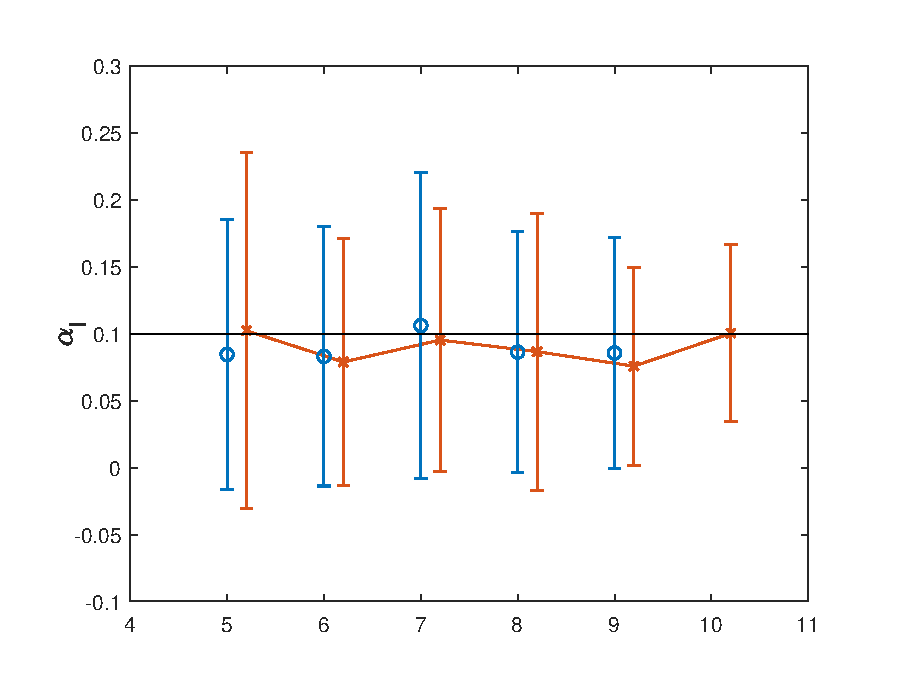
\includegraphics[width=1\textwidth]{images/alpha_I.eps}
\end{minipage}}
\subfigure[$\alpha_B$ Latent]{
\begin{minipage}[t]{0.235\textwidth}
  \centering
  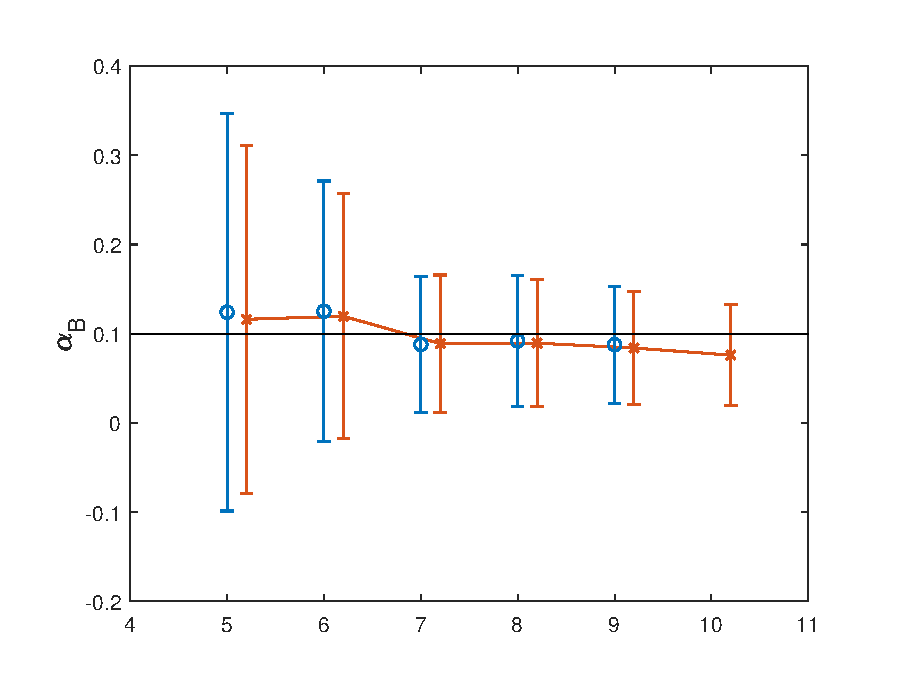
\includegraphics[width=1\textwidth]{images/alpha_B.eps}
  \end{minipage}}
\subfigure[$l$ Latent]{
\begin{minipage}[t]{0.235\textwidth}
 \centering
  \includegraphics[width=1\textwidth]{images/l.eps}
\end{minipage}}
\subfigure[$\sigma$ Latent]{
\begin{minipage}[t]{0.235\textwidth}
  \centering
  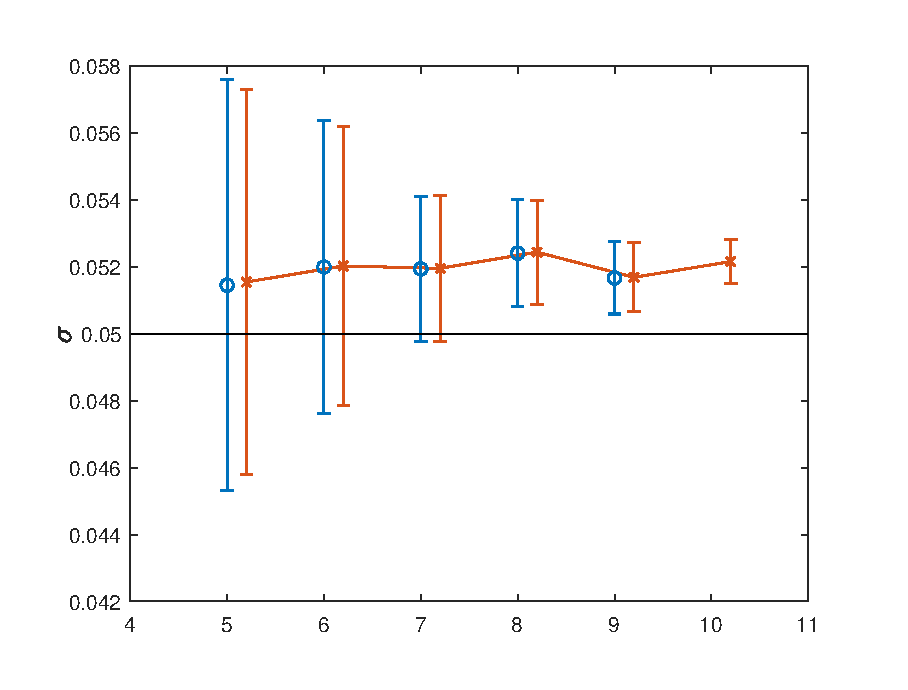
\includegraphics[width=1\textwidth]{images/sigma.eps}
  \end{minipage}}\\
\subfigure[$\alpha_I$ Joint]{
\begin{minipage}[t]{0.235\textwidth}
 \centering
  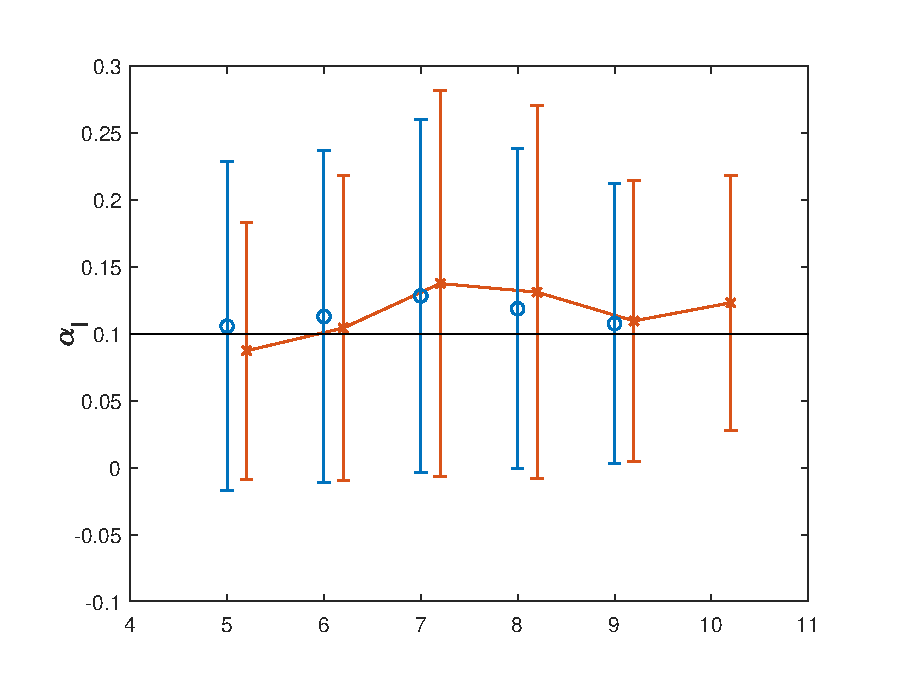
\includegraphics[width=1\textwidth]{images/alpha_I_joint.eps}
\end{minipage}}
\subfigure[$\alpha_B$ Joint]{
\begin{minipage}[t]{0.235\textwidth}
  \centering
  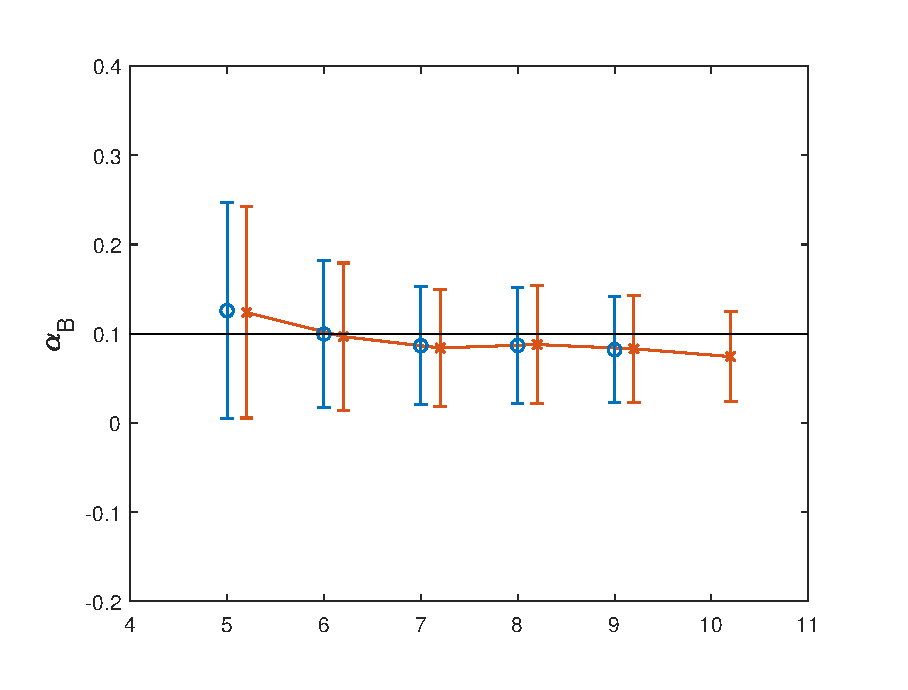
\includegraphics[width=1\textwidth]{images/alpha_B_joint.eps}
\end{minipage}}
\subfigure[$l$ Joint]{
\begin{minipage}[t]{0.235\textwidth}
 \centering
  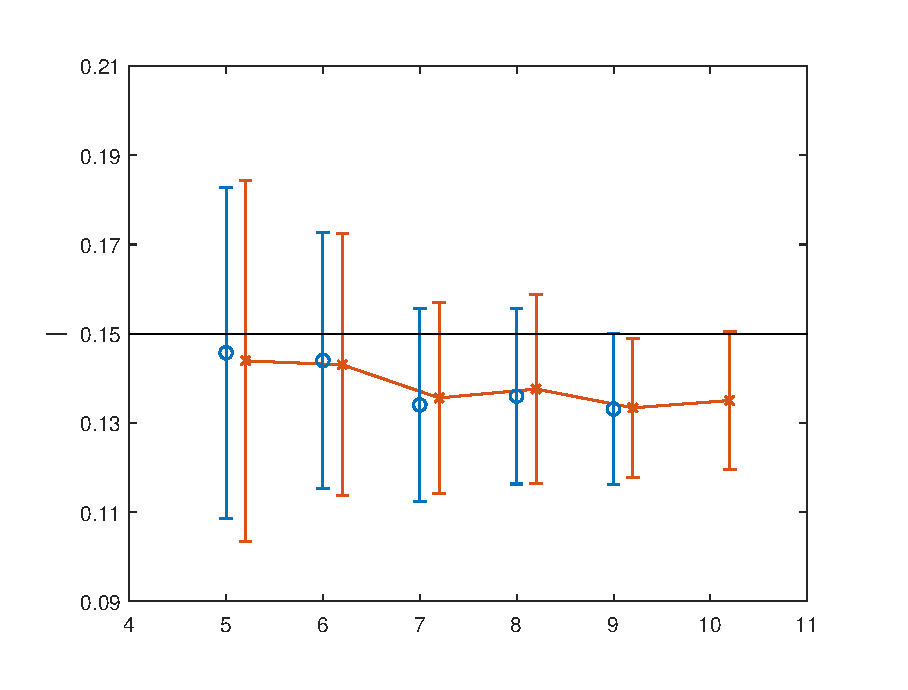
\includegraphics[width=1\textwidth]{images/l_joint.eps}
\end{minipage}}
\subfigure[$\sigma$ Joint]{
\begin{minipage}[t]{0.235\textwidth}
  \centering
  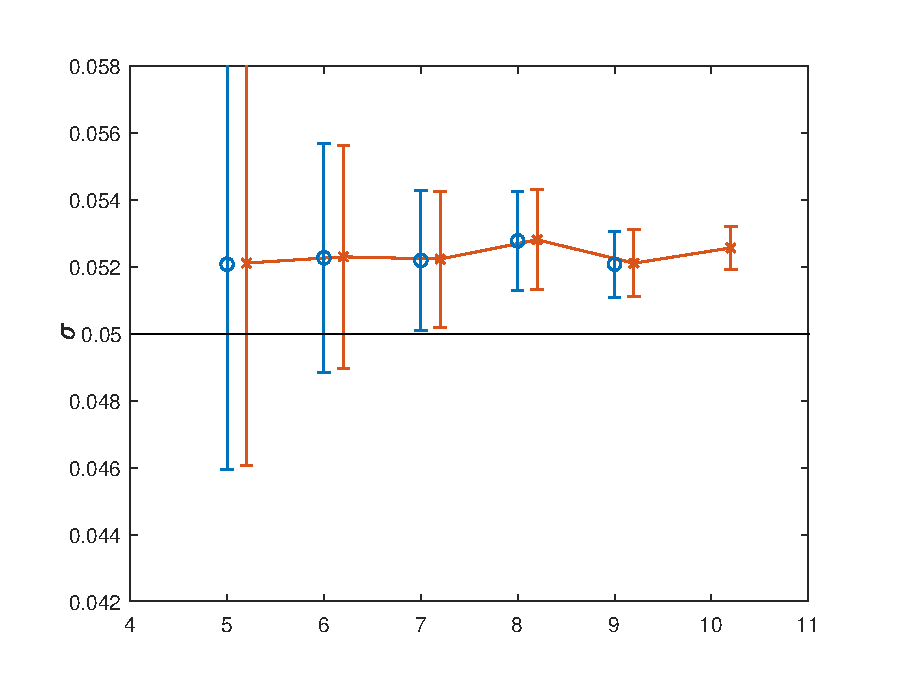
\includegraphics[width=1\textwidth]{images/sigma_joint.eps}
\end{minipage}}
\caption{Parameter estimations and corresponding 95\% confidence intervals computed via the expected Fisher information matrix. We solve the nonlinear system of score equations \eqref{eq41},\eqref{eq51} using the physics-based covariance model with the number of mesh points $k=2^q$ in each dimension for $q$ ranging from $5$ to $10$. Red lines with crosses represent MLE using low-rank approximations. The first row describes the results for latent process MLE \S \ref{sec:41}. The second row describes the results for joint process MLE \S \ref{sec:42}. MLE results using exact score equations are provided for $q=5$ to $9$ by using blue lines with circles. For $q=10$ the exact MLE calculation ran out of memory.} \label{fig:1}
\end{figure}

\subsubsection{Comparison of Covariance Models}\label{sec:512}
\par We now examine the predictive performance of the physics-based covariance model \S \ref{sec2}, inclusive of the low-rank \S \ref{sec:lra} and implicit formulation 
approximation \S \ref{sec:ajh} effects. We compare the latent process kriging \S \ref{sec:lpf} and joint process kriging \S \ref{sec:jpf} with independent process kriging, which ignores the relations between the two processes by removing the cross-covariance. The latter setup aims to exhibit the features of the most prevalent approaches in modeling where a difficulty of expressing valid cross-covariances models results in the need for modeling different observables independently. 
~\\
\par \textbf{Independent kriging.} In this setting we separate the output and latent processes by considering their covariances independently and setting the cross-covariance to zero. We use the following covariance structure:
\begin{align}
    K_{11}=\begin{pmatrix}\mathrm{Cov}(y_{o},y_{o})+\sigma^{2}I_{d} & 0\\0 & {\rm{Cov}}(z_{o},z_{o})+\sigma^{2}I_{D}\end{pmatrix},\label{eq65}
\end{align}
\begin{align}
    K_{21}=\begin{pmatrix}\mathrm{Cov}(y_{p},y_{o}) & 0\\0 & {\rm{Cov}}(z_{p},z_{o})\end{pmatrix},\label{eq66}
\end{align}
\begin{align}
    \mathcal{M}_{\mathrm{ind}}=\begin{pmatrix}m(y_{p})\\m(z_{p})\end{pmatrix}+(K_{21})(K_{11})^{-1}\begin{pmatrix}y_{o}-m(y_{o})\\z_{o}-m(z_{o})\end{pmatrix}.\label{eq67}
\end{align}
At this stage the ideal comparison would be with a well-chosen Gaussian kernel to model $\mathrm{Cov}(y_{o},y_{o})$ and ${\rm{Cov}}(z_{p},z_{o})$ separately. 
Since our model originates in the approximation of a nonlinear equation, the implied covariance of the linearized process for meaningful boundary conditions will not be stationary (since the advection would depend on space). Modeling a nonstationary process in the output space is a difficult endeavor with no simple approach (other than using a simple stationary kernel class, e.g., a squared exponential \cite{GPforML}). Since our focus is on understanding the effect of ignoring covariance and getting access to a model that is reasonable and easy to set up, we still use the physics-based covariance model $\mathrm{Cov}(y_{o},y_{o})=L_{o}\mathrm{Cov}(z,z)L_{o}^{T}$ and $\mathrm{Cov}(y_{p},y_{o})=L_{p}\mathrm{Cov}(z,z)L_{o}^{T}$, where $L_{o}$, $L_{p}$ correspond to the Jacobians of mapping $F_{o}$, $F_{p}$, respectively. Thus, we consider the effect of $z$ on $y$ for the purpose of the autocovariance but not for the purpose of the cross-covariance. While it would be more principled to set up a model that completely ignores the physics, we believe that using the ``best model'' for the auto-covariance in this circumstance  allows us to sharply assess the effects of ignoring the cross-covariance, an approach also used in the paper that inspired this work \cite{CovModel}. Moreover, this does not affect the main concern of our paper, namely, whether the approximation we use to make the computation scalable still presents enough accuracy overall. 

We note that if we made this choice, the prediction carried out by \eqref{eq67} would be identical to the latent process approach \S \ref{sec:lpf}, provided that the parameters $\theta$ stay the same. Since, however, in the case of the model $\eqref{eq65}-\eqref{eq66}$ we use both $z_o$ and $y_o$ data to estimate $\theta$, whereas for the latent process model in  \S \ref{sec:lpf} we use only $y_o$, the parameters $\theta$ and thus the kriging results will be different. The joint process approach from \S \ref{sec:jpf}, however, will use values of both $y_o$ and $z_o$ both for estimating $\theta$ and for kriging. 

We consider a model using the joint process covariance model structure \eqref{eq23}-\eqref{eq25} with the hyperparameters defined above \eqref{eq:true_parameter} that were used to produce the data (the ``true'' parameters). We denote this true model by $\mathcal{M}_{*}$. 

We then take a fixed mesh size with $k=200$, which results in a total of $40,000$ data points for the numerical approximation of PDE using \eqref{eq60}. We randomly pick $d=400$ data points in the output field $w$ as observations $y_{o}$, which corresponds to 1\% of the total field to observe. In the joint process case \S \ref{sec:jpf}, we have $D=20$ additional observations each from the initial conditions and boundary conditions as latent observations $z_{o}$, which are $10\%$ of the latent variables. Note that the dimension of $w$ is roughly the square of the dimension of $z$, so the dimension of the observations of $z$ and $w$ are comparable. Note also that the setting is similar to \cite{CovModel}. 

Since the computational complexity is not a major concern in this subsection, we predict the entire remaining field $y_{p}=w\setminus y_{o}$ and $z_{p}=z\setminus z_{o}$. We first generate one sample using the hyperparameters \eqref{eq:true_parameter}, termed the calibration sample, which is used to fit the covariance models $\mathcal{M}_{1}$ \eqref{eq18}, $\mathcal{M}_{2}$ \eqref{eq23}-\eqref{eq25},$\mathcal{M}_{\mathrm{ind}}$ \eqref{eq65}-\eqref{eq67} as described in \S \ref{sec:511}. Then we further generate 50 independent samples used for tests in our experiment, termed validation samples. The results are averaged and summarized in the upper block of Table \ref{table:1}.

\par We note that the RMS error on $y_p$ of the three physics-based covariance models $\mathcal{M}_{1}$, $\mathcal{M}_{2}$ and $\mathcal{M}_{*}$ is significantly smaller (by a factor of at least 6) on the validation samples than the error of the independent kriging $\mathcal{M}_{\mathrm{ind}}$, which demonstrates the contribution of the cross-covariance terms to the predictions. Furthermore, the two models using joint process kriging $\mathcal{M}_{2}$ and $\mathcal{M}_{*}$ have similar performance and are both better by about $10\%$ on the validation samples compared with the latent process kriging $\mathcal{M}_{1}$ because of the additional information conveyed by the observations $z_{o}$. This improved accuracy occurs despite the fact that we have low-rank \S \ref{sec:lra},  differentiation \S \ref{sec:ajh} and linearization approximation errors in the computation of the covariance. While our starting the MLE at the true parameters allows for the possibility of other local minima,  the approximated likelihood has minima that are mostly indistinguishable from the true parameters for the purpose of the accuracy of the kriging. 

\begin{table}[!t]
\centering
 \caption{Predictive RMS Error (excluding observed locations). The observation density is $1\%$ for $w$ and $10\%$ for $z$, although the dimension of the observation vectors is comparable. The observations are chosen randomly in the field. The predictions are conducted for all the remaining field in $w$ and $z$ except the observed positions. The first four rows contain covariance models without higher-order terms from \S \ref{sec:512}, and the last three rows contain covariance models with higher-order terms from \S \ref{sec:513}.}\label{table:1}
\begin{tabular}{|c|c|c|c|c|}
\hline
 & \multicolumn{2}{c}{Validation Samples} & \multicolumn{2}{|c|}{Calibration Sample}\\
 \hline
 Models  & $y_{p}$ & $z_{p}$ & $y_{p}$ & $z_{p}$\\
\hline
\hline
$\mathcal{M}_{1}$  & 0.0241 & - & 0.0296 & - \\
\hline
$\mathcal{M}_{2}$  & 0.0211 & 0.0401 & 0.0195 & 0.0495 \\
\hline
$\mathcal{M}_{\mathrm{ind}}$  & 0.1422 & 0.4780 & 0.1189 & 0.5107 \\
\hline
$\mathcal{M}_{*}$  & 0.0211 & 0.0339 & 0.0195 & 0.0514 \\
\hline
\hline
$\mathcal{M}_{1}^{+}$  & 0.0228 & - & 0.0247 & - \\
\hline
$\mathcal{M}_{2}^{+}$ & 0.0180 & 0.0334 & 0.0175 & 0.0325 \\
\hline
$\mathcal{M}_{*}^{+}$ & 0.0207 & 0.0331 & 0.0117 & 0.0335 \\
\hline
\end{tabular}
\end{table}



\subsubsection{Correction of Nonlinearity}\label{sec:513}
\par Since the Burger's equation is nonlinear, we now consider adding higher-order terms in the covariance model to account for the nonlinear behaviors generated by the equation using the methods described in \S \ref{sec33}. To demonstrate the benefit gained from the higher-order terms, we consider the same experiment settings as in Section \ref{sec:512}. Note that we  consider the correction of nonlinearity only on models $\mathcal{M}_{1}$, $\mathcal{M}_{2}$, and $\mathcal{M}_{*}$. The models with higher-order terms included are denoted by $\mathcal{M}_{1}^{+}$, $\mathcal{M}_{2}^{+}$, and $\mathcal{M}_{*}^{+}$, respectively. Specifically, $\mathcal{M}_{1}^{+}$ follows the latent process kriging with higher-order terms in Algorithm \ref{alg:3}. $\mathcal{M}_{2}^{+}$ and $\mathcal{M}_{*}^{+}$ follow the joint process kriging with higher-order terms in Algorithm \ref{alg:6}. When setting the parameters $\theta=(\alpha_{I},\alpha_{B},l,\sigma)$ in $\mathcal{M}_{1}^{+}$ and $\mathcal{M}_{2}^{+}$, we use the parameters fitted by the approximated MLE described in \S \ref{sec4} but for the linear approximation process only, that is, the same process described in \S \ref{sec:511} (in other words we consider the nonlinearity when kriging but not when carrying out MLE). In contrast, for $\mathcal{M}_{*}^{+}$ we use the true parameters \eqref{eq:true_parameter}. The performance of the nonlinearly corrected models on the same calibration sample and validation samples is summarized in the lower block of Table \ref{table:1}. We note that the performance of all three models is better, albeit marginally in most cases (in the $2 \% -- 14 \%$ range), than their counterparts using covariance models without higher-order terms $\mathcal{M}_{1}$, $\mathcal{M}_{2}$, and $\mathcal{M}_{*}$ because the higher-order terms help account for the nonlinearities. The improvement is the largest in the joint model $\mathcal{M}_{2}$ to the point where it exceeds the one with the true parameters. It is unlikely that this situation will hold for all possible experimental validation setups, but the improvement in RMSE is clear across all models when considering nonlinear effects, even if small. 
\par Additionally, to provide a visual comparison of the predictions, we combine the predicted data and the observations to reconstruct the whole field $w$. To demonstrate the effectiveness of the higher-order terms, we compute the average error distribution over the 50 validation samples for joint process kriging models $\mathcal{M}_{2}$ and $\mathcal{M}_{2}^{+}$. The comparison is shown in Figure \ref{fig:2}. As we can observe, even if the reduction in RMSE is not large, the pattern of the error is much improved. The error is uniformly smaller for covariance models with higher-order terms (which indicates that in the max norm the error improvement is significant), which demonstrates the usefulness of the nonlinear correction. To support this observation, we report quartiles to describe the distribution of the error surface. The three quartiles ($Q_{1},Q_{2},Q_{3}$) of the error are $0.078$, $0.0109$, and $0.0153$ for model $\mathcal{M}_{2}$ in Figure \ref{fig:2}(a). In contrast, the three quartiles for model $\mathcal{M}_{2}^{+}$ in Figure \ref{fig:2}(b) are $0.067$, $0.082$, and $0.0102$. Therefore the spatial distribution of the error has a much thinner tail for model $\mathcal{M}_{2}^{+}$ compared with model $\mathcal{M}_{2}$; indeed  the third quartile of the error for $\mathcal{M}_{2}^{+}$ is smaller by about a third compared with the third quartile of the error for $\mathcal{M}_{2}$.
%% \cm{Probably looking at the max error and not RMSE may help here} \YC{My idea was to use the RMSE in the table to show an averaged performance improvement and use Fig.\ref{fig:2} to illustrate %% the difference between error distribution. Actually one can directly observe the max error in two cases by Fig.\ref{fig:2} because the colorbars have the same range. There are dark red areas in %%(a) but not in (b). If it is not clear, I can add something like an error histogram. I also report the three quartiles in teal color}

\begin{figure}[!t]
\subfigure[Without higher-order terms]{
\begin{minipage}[t]{0.5\textwidth}
 \centering
  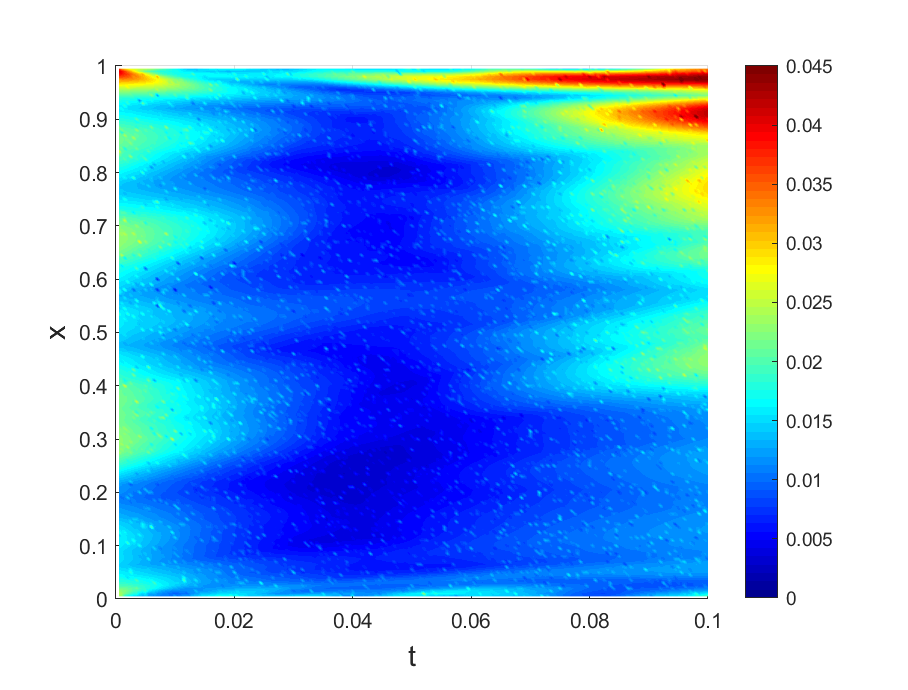
\includegraphics[width=1\textwidth]{images/error_heatmap_M3.eps}
\end{minipage}}
\subfigure[With higher-order terms]{
\begin{minipage}[t]{0.5\textwidth}
  \centering
  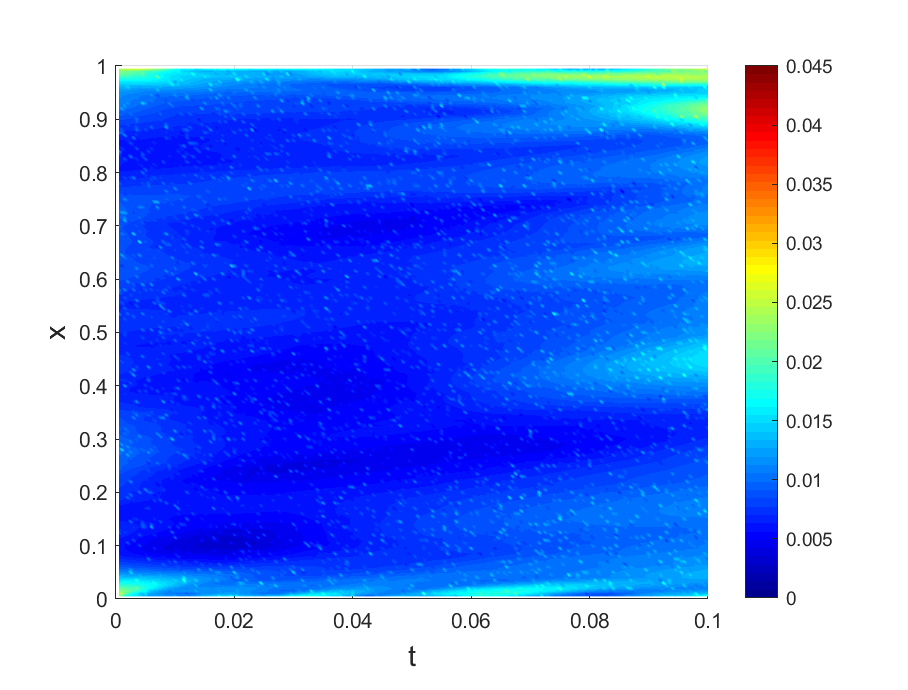
\includegraphics[width=1\textwidth]{images/error_heatmap_M3plus.eps}
  \end{minipage}}
  \caption{Error distribution of the predicted field compared with the true data \S \ref{sec:513}. \textbf{Left}: Results from joint process kriging $\mathcal{M}_{2}$. The covariance model follows \eqref{eq23}-\eqref{eq25}, which includes up to second-order terms corresponding to \eqref{eq4}. \textbf{Right}: Results from joint process kriging with higher-order terms $\mathcal{M}_{2}^{+}$. The covariance model follows \eqref{eq:jntnlnkrg}-\eqref{eq:jntnlnk21}, which includes up to fourth-order terms corresponding to \eqref{eq5}\eqref{eq6}. The higher-order terms should account for part of the nonlinear behavior of Burger's equation.}\label{fig:2}
\end{figure}

\subsubsection{Demonstrating Quasilinear Scaling}\label{ss:quasilinear}
 We now present numerical experiments to demonstrate the scalability of our proposed approach when computing the covariance parameters $\theta$ by the maximum likelihood approach in the \S \ref{sec:511} setting. Specifically, we carry out the computation of the approximated score equations \S \ref{sec4}, followed by the kriging procedures described in \S \ref{sec3} to predict the field of interest at prescribed points. To vary the size of the problem, we take mesh size $k=2^{q}$ for $q$ ranging from $10$ to $14$. We randomly observe $d=3k$ data points from the output process $w$ and $D=1.5k$ data points from the latent process $z$. Then we predict $3k$ points for the output process and $1.5k$ points for the latent process at sites that are also randomly chosen. The random part of our experiment is repeated 50 times. For both latent process kriging \S \ref{sec:lpf} and joint process kriging \S \ref{sec:jpf}, we compare the average time cost over the 50 of our workflow without higher-order terms (Algorithm \ref{alg:1}\&\ref{alg:2}) and with higher-order terms (Algorithm \ref{alg:3}\&\ref{alg:6}). For the latent process MLE \S \ref{sec:41}\ and joint process MLE \S \ref{sec:42}, we compare the time of solving the approximated score equations \eqref{eq41} and \eqref{eq51} with the time of solving the exact ones (where the covariance matrices are exactly computed and not approximated by interpolation); the timings reported are for  the computation on the first sample only. The results are summarized in Figures \ref{fig:3_1} and \ref{fig:3_2}. Lines corresponding to the theoretical scaling $O(k\log^{2}{k})$ are added to each plot to demonstrate the quasilinear scaling of our approaches.

 As we can observe, the scaling of the proposed approximated approaches in latent and joint process kriging follow the $O(k\log^{2}{k})$ theoretical line. Comparing the algorithm with and without higher-order terms, we observe that the algorithm without higher-order terms scales slightly better because of the extra operations when considering higher-order terms. This effect will be alleviated as the datasets grow larger. For the score equations computation and Fisher information matrix estimation, the quasilinear scaling is clearly demonstrated in Figure \ref{fig:3_2}. Note that our approximated approach requires stochastic estimation of the trace term, which is not as efficient as direct computation in small datasets, namely, $q=10$ in Figure \ref{fig:3_2}.
 
In summary, for the synthetic data case 
we conclude that our approach scales quasilinearly \S \ref{ss:quasilinear}, that the approximations that we have proposed  still allow an accurate recovery of the parameters defining the shape of the uncertainty \S \ref{sec:511}, that the accurate treatment of the cross-covariance significantly improves prediction \S \ref{sec:512}, and that  including the nonlinear corrections in the covariance slightly improves the RMSE of the prediction but may significantly help with removing complex error artifacts \S \ref{sec:513}.

\begin{figure}[!t]
\centering
\subfigure[Time for latent process kriging]{
\begin{minipage}[t]{0.30\textwidth}
 \centering
  \includegraphics[width=1.1\textwidth]{images/M1_time_2.eps}
\end{minipage}}
\subfigure[Time for joint process kriging]{
\begin{minipage}[t]{0.30\textwidth}
  \centering
  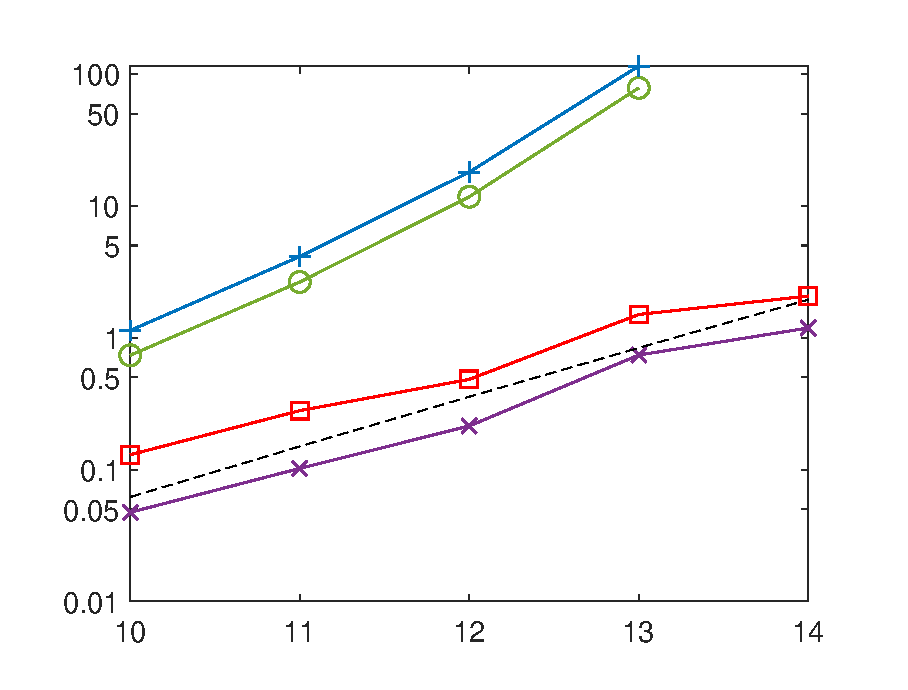
\includegraphics[width=1.1\textwidth]{images/M2_time_2.eps}
  \end{minipage}}\\
  \caption{Times taken (in seconds) to solve the GP regression problem by (a) latent process kriging (Algorithm \ref{alg:1}\&\ref{alg:3}) and (b) joint process kriging (Algorithm \ref{alg:2}\&\ref{alg:6}). We present the time to compute latent/joint process kriging without higher-order terms exactly (circle) and approximately (square) and latent/joint process kriging with higher-order terms exactly (plus) and approximately (cross). All results are averaged over 50 tests. Note that the y-axis is in logarithmic scale. The lines corresponding to theoretical $O(k\log^{2}{k})$ scaling (dash lines) are added to each plot.}\label{fig:3_1} 
\subfigure[Time for estimating latent \& Joint process score equations]{
\begin{minipage}[t]{0.30\textwidth}
 \centering
  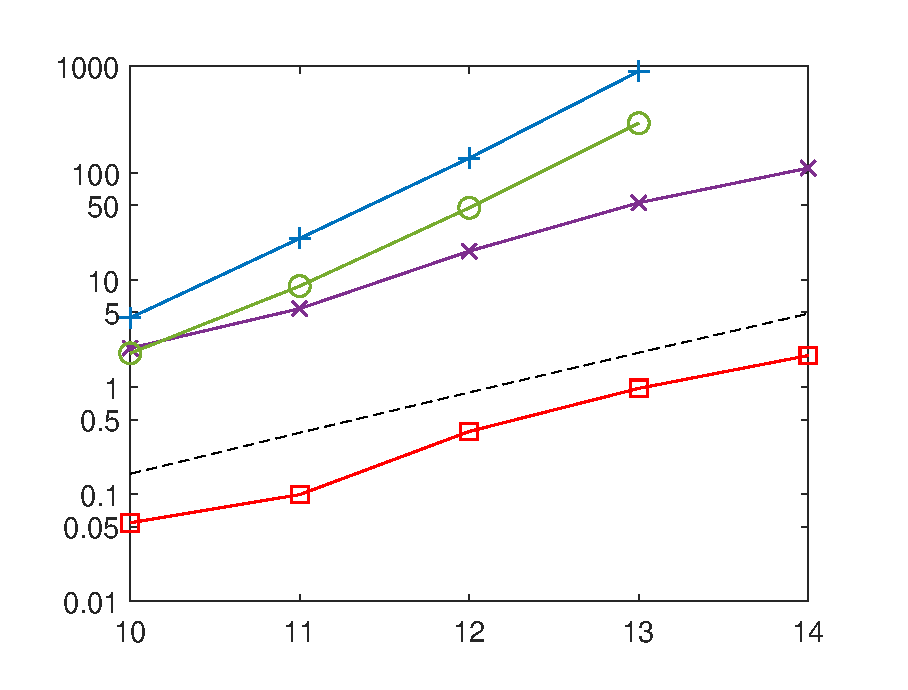
\includegraphics[width=1.1\textwidth]{images/Score_time_2.eps}
\end{minipage}}
\subfigure[Time for estimating the Fisher information matrix]{
\begin{minipage}[t]{0.30\textwidth}
 \centering
  \includegraphics[width=1.1\textwidth]{images/f_time_2.eps}
\end{minipage}}
  \caption{Times taken (in seconds) to evaluate (a) latent and joint process score equations (Algorithm \ref{alg:4}\&\ref{alg:5}) and (b) the expected Fisher information matrix via equation \eqref{eq:latent}, \eqref{eq:joint}. For both plots, we present the time to evaluate the score equations or the expected Fisher information matrix for latent process exactly (circle) and approximately (square) and for joint process exactly (plus) and approximately (cross). All results are averaged over 50 tests. Note that the y-axis is in logarithmic scale. The lines corresponding to theoretical $O(k\log^{2}{k})$ scaling (dash lines) are added to each plot.} 
  	%%\cm{Probably the longest caption of a figure I \textit{ever read}. It is also very hard to follow. You need to insert brief legends in upper left and reduce the caption} \YC{I feel the legends may become too long for each plot. So I separate them to two plots FIG.3 and 4. Hopefully it looks better. }
  	\label{fig:3_2} 
\end{figure}
 				

\subsection{Real Data Experiment}\label{ss:rde}
\par In this subsection, we consider realistic climate observation data and a simple tropical climate model connecting key quantities as the physical information we will use to inform our covariance model. The model equation is given by
\begin{align}
    \frac{\partial w}{\partial t}=-\tilde{Q}\nabla u - \frac{1}{\tau_{w}}w+b_{w}\nabla^{2}w+D_{w}\dot{W},\label{eq68}
\end{align}
where $u$ is the first baroclinic mode of the zonal wind velocity anomalies, $w$ is the water vapor anomalies in middle troposphere, and $\dot{W}$ is Gaussian white noise. The core dynamic \eqref{eq68} uses a modified equation from \cite{stechmann2017unified}. The term $-\tilde{Q}\nabla u$ is a traditional model of convective adjustment of water vapor caused by wind. The term $- \frac{1}{\tau_{w}}w$ accounts for moisture sink associated with deep convection and precipitation. $b_{w}\nabla^{2}w$ represents the diffusion of water vapor, and $D_{w}\dot{W}$ represents stochastic forcing. In short, this model represents the effect of precipitation, natural diffusion, and turbulent advection in a simplified, linearized form. Besides the deterministic dynamic components, the stochastic moisture forcing is, in part, representative of mesoscale convective processes that are not
represented by the larger-scale dynamics in \eqref{eq68}. Therefore one can reasonably assume that such processes are approximately spatiotemporally uncorrelated. The parameter values $\tilde{Q}=0.45$, $\tau_{w}=3.99$, $b_{w}=0.7$, and $D_{w}=0.003$ are all dimensionless and are suggested by \cite{stechmann2017unified}.
\par To numerically solve the model \eqref{eq68}, we use the initial condition $w_{0}$ and random field $u$ as model inputs with periodic boundary condition. The equation can be solved by using the Euler-Maruyama method \cite{kloeden2013numerical} and also in Fourier space \cite{appliedSDE}. We recommend  solving in Fourier modes since a semi-analytical solution \cite{appliedSDE} exists for each Fourier mode and can significantly reduce the time cost of numerical simulation.
\par To apply our framework, we numerically solve $w$ as output process, and we treat the concatenation of the initial condition $w_{0}$, the random process $u$, and $\dot{W}$ as the latent process of our framework, in other words, $z^{T}=(w_{0}^{T},u^{T})$ in our framework \S \eqref{eq16}-\eqref{eq17}. Similar to \S \ref{sec:51}, we define $w=G(z)$, where $w$ is the solution produced by semi-analytical solver of stochastic differential equation \eqref{eq68}. In the following test, we denote $y_{o}$ as the observed subset of $w$, which  includes additional observation noise, and $y_{p}$ as another subset that is going to be predicted. The mappings $F_{o}$, $F_{p}$ required by our setup \eqref{eq16}-\eqref{eq17} are obtained by corresponding components of mapping $G$.


\subsubsection{Data Source and Data Processing}\label{sec:521}
\par To associate the model \eqref{eq68} with a suitable real dataset, we argue that the zonal wind velocity serves as a natural surrogate of $u$ and that the relative humidity (mixing ratio) in 500 hPa pressure level is a common surrogate of the water vapor $w$ in middle troposphere. 

\par The data source we used here is the National Centers for Environmental Prediction–National Center for Atmospheric Research (NCEP\--NCAR) reanalysis project \cite{kalnay1996ncep}. The daily zonal wind velocity and relative humidity data are used. Both datasets have a spatial resolution of $2.5^{\circ}\times2.5^{\circ}$ and a daily temporal resolution from 1 January 1979 to 31 December 2011. The connections between model variables and observations are largely based on previous work \cite{stechmann2014walker,stechmann2015identifying,ogrosky2016identifying}.

\par The influence of seasonal cycle has been removed from both datasets, and a further 120-day mean of previous 120-day signals is subtracted, as is recommended by the Climate Variability and Predictability program \cite{waliser2009mjo}. Then both datasets are projected to the parabolic cylinder functions, and only the first meridional mode is used. This step converted the two-dimensional spatial data to one dimensional, which facilitates our computation. Then the datasets have two dimensions remaining (one spatial dimension and one temporal dimension). Furthermore, we treat the observation data as true signals and generate artificial observations by adding independent Gaussian noise $\epsilon_{w}\sim \mathcal{N}(0,\sigma_{w}^{2}I)$ and $\epsilon_{u}\sim \mathcal{N}(0,\sigma_{u}^{2}I)$ to water vapor data $w$ and zonal wind velocity data $u$, respectively. Parameters $\sigma_{w}$ and $\sigma_{u}$ are taken to be $15\%$ of the standard deviation of each true signal, similar to other previous studies (e.g., \cite{chen2016filtering}).

\par Note that the real data are normalized to have the same variance as the model data before using. This approach differs from \cite{stechmann2017unified}, where the data are nondimensionalized using the standard equatorial reference scale \cite{stechmann2015identifying} because here we use anomalies in our modified model equation. For more detailed raw data preprocessing methods see \cite{stechmann2015identifying}. In Figure \ref{fig:4} we show the observational relative humidity data for all longitudes from Dec. 1982 to April 1983.

\begin{figure}[!t]
  \centering
  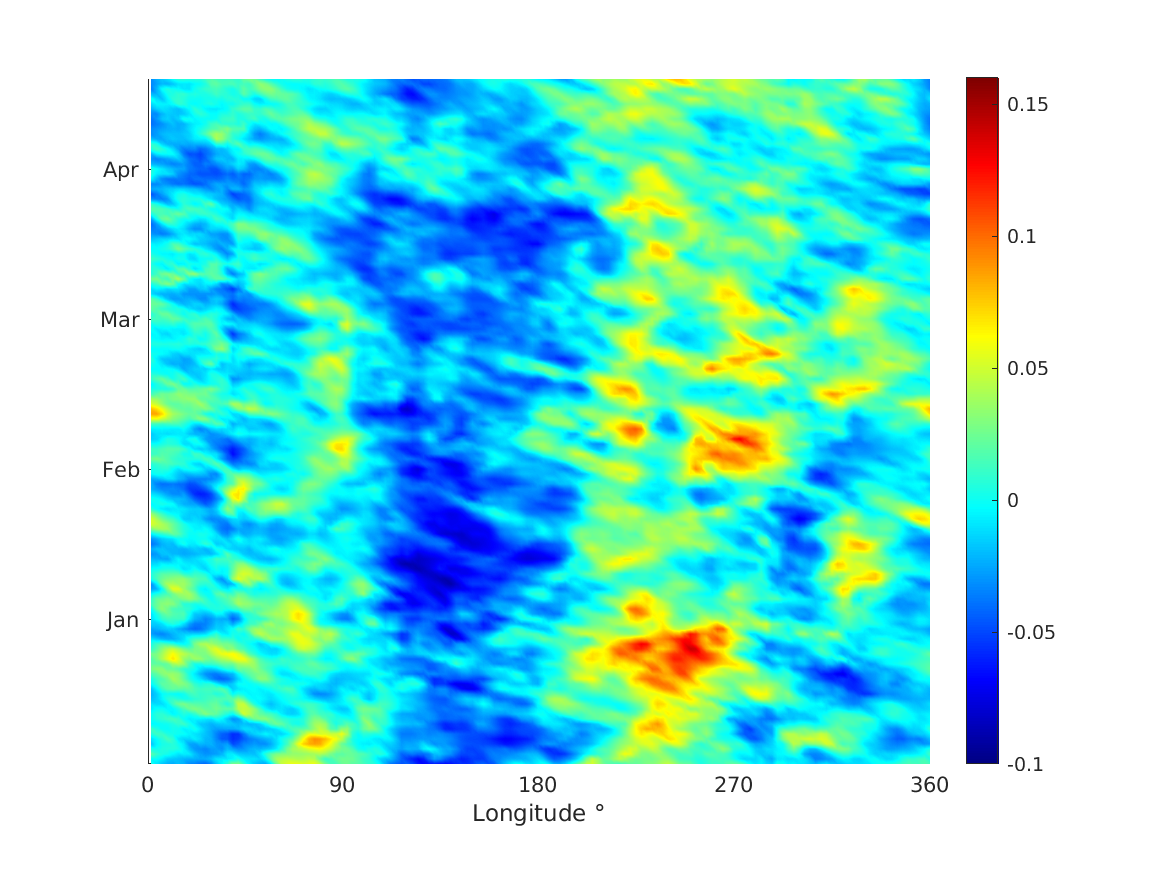
\includegraphics[width=0.4\textwidth]{images/q_sample_1.eps}
  \caption{Observations of relative humidity at 500 hPa pressure level. The time period is from Dec. 1, 1982 to April 18, 1983. The data have been nondimensionalized.}\label{fig:4}
\end{figure}

\subsubsection{End-to-End Numerical Tests}
\par We combine our proposed scalable MLE parameter estimation and GP regression together and test their performance. 
%%\cm{You must be clear here what are your paramters $\theta$ here. Do you include all the ones above or do you assume some known?} \YC{I'm planning to first introduce the covariance models here and discuss about parameters in $\mathrm{Cov}(z,z)$ in \eqref{eqn1}, \eqref{eqn2}}. 
Four  covariance structures are compared here. The latent process kriging $\mathcal{M}_{1}$ \eqref{eq18} and the joint process kriging $\mathcal{M}_{2}$ \eqref{eq23}-\eqref{eq25} follow the same design as we discussed in \S \ref{sec3}. Additionally the joint independent kriging $\mathcal{M}_{\mathrm{ind}}$ ignores the cross-covariance between the latent process $z$ and the output $w$ and is formulated as follows:

\begin{align}
    K_{11}=\begin{pmatrix}\mathrm{Cov}(y_{o},y_{o})+\sigma_{w}^{2}I & 0\\0 & {\rm{Cov}}(z_{o},z_{o})+K_{\epsilon_{z}}\end{pmatrix},\label{eq69}
\end{align}
\begin{align}
    K_{21}=\begin{pmatrix}\mathrm{Cov}(y_{p},y_{o}) & 0\\0 & {\rm{Cov}}(z_{p},z_{o})\end{pmatrix},\label{eq70}
\end{align}
\begin{align}
    \mathcal{M}_{\mathrm{ind}}=m(y_{p})+(K_{21})(K_{11})^{-1}\begin{pmatrix}y_{o}-m(y_{o})\\z_{o}-m(z_{o})\end{pmatrix},\label{eq71}
\end{align}
where $z_{o}$ consists of an observed subset of the components of the latent process $z$ and $z_{p}$ consists of another subset that is to be predicted. $K_{\epsilon_{z}}$ is the observation noise covariance matrix. Since $z$ is a concatenation of initial value $w_{0}$ and wind velocity field $u$, $K_{\epsilon_{z}}$ is block-diagonal with Gaussian observation noise covariance matrices in its diagonal blocks. Similar to the approach in  \S \ref{sec:512}, we use the physics-based covariance model $\mathrm{Cov}(y_{o},y_{o})=L_{o}\mathrm{Cov}(z,z)L_{o}^{T}$ and $\mathrm{Cov}(y_{p},y_{o})=L_{p}\mathrm{Cov}(z,z)L_{o}^{T}$, where $L_{o}$, $L_{p}$ correspond to the Jacobians of mapping $F_{o}$, $F_{p}$, respectively. The computation involving the three models is carried out bt using  low-rank approximations. We include kriging using the exact joint process covariance model \eqref{eq23}-\eqref{eq25} but without low-rank approximations as contrast. We denote this exact joint process kriging model as $\mathcal{M}_{e}$.

\par For all the covariance models $\mathcal{M}_{1}$, $\mathcal{M}_{2}$, $\mathcal{M}_{\mathrm{ind}}$, and $\mathcal{M}_{e}$ used here, each component of the latent process $z$ is modeled by a Gaussian process with square exponential covariance function. In other words, we assume
\begin{align}
    &w_{0}\sim\mathcal{N}(m(w_{0}),\alpha_{w}\mathrm{exp}(-\frac{r^{2}}{2l_{w}^{2}})),\label{eqn1}\\ &u\sim\mathcal{N}(m(u),\alpha_{u}\mathrm{exp}(-\frac{r^{2}}{2l_{u}^{2}})),\label{eqn2}
\end{align}
with magnitude parameters $\alpha_{w} and\alpha_{u}$ and length scale parameters $l_{w},l_{u}$. Let $\theta=(\alpha_{w},\alpha_{u},l_{w},l_{u})$  be the unknown parameters that we will estimate; we assume that the other parameters, including model parameters in \eqref{eq68} and observation error covariance, are known and specified at the beginning of \S \ref{ss:rde} based on \cite{stechmann2017unified}. All four parameters will be estimated from the observation data via score equations.
%% \cm{Need to be clear again whether these are the only parameters you calibrate. If by this you mean that $\theta=(\alpha_{w},\alpha_{u},l_{w},l_{u})$ and all other parameters are assumed known you need to be clear about it. I am particularly concerned by $D_w$ as this is an error term and there is not a good basis to get it from physical principles}. \YC{I add one sentence to hopefully clarify the parameters to be estimated (on the top of page 22 in teal color)}

\par The processed relative humidity observation data are divided into different time snapshots with equal lengths. Each snapshot has $144\times 140$ grid points (20,160 data points) that represent 144 longitudes each day and an 140-day time window. First we randomly pick one snapshot field as the calibration sample for parameter fitting. For models $\mathcal{M}_{1}$, $\mathcal{M}_{2}$, and $\mathcal{M}_{\mathrm{ind}}$, we use scalable latent and joint process MLE described in \S \ref{sec4}. For model $\mathcal{M}_{e}$, we directly evaluate the score equations without approximations. The fitted parameters are used in the following kriging processes. The validation samples are chosen to be snapshots of the same size but at least 120 days away from the calibration sample, which can help remove the effect of the trend of most intraseasonal oscillations. Numerical results are summarized in Table \ref{table:2}. We observe that  the approximation we made to the likelihood does not result in a significant kriging error, by comparing the  validation sample performance of $\mathcal{M}_{1}$, $\mathcal{M}_{2}$, and $\mathcal{M}_{e}$ models whose performance is indistinguishable (despite the fact that model $\mathcal{M}_{e}$ is more expensive and not scalably computable). We also observe that ignoring the covariance structure reduces the performance of the $\mathcal{M}_{ind}$ by about $20\%$. Therefore our approximation ensures scalability at a negligible cost to the accuracy, and the accurate modeling of the cross-covariance pays off in accuracy improvements for real data. 
 
\par To provide a visual representation of the results, we illustrate in Figure \ref{fig:5} the relative humidity predictions on the calibration sample using model $\mathcal{M}_{2}$ and $\mathcal{M}_{\mathrm{ind}}$. The predicted time window is Dec. 1982 to April 1983, which is the same as observations in Figure \ref{fig:4}. In Figure \ref{fig:6} we show histograms of the predictive errors of the two models, respectively. Note that the vertical axis represents the probability density of a certain error range in logarithmic scale. For bars with zero probability, we truncate the logarithm and set it as the base value of the bar plot in order to prevent it from approaching negative infinity. As a result, the zero probability bars are also of height zero. We  observe that the prediction error is reduced and has thinner tails when using the physics-based covariance models $\mathcal{M}_{1}$, $\mathcal{M}_{2}$, and particularly so for the latter. 

%%\cm{Completely unclear. I think you should show the histograms of the errors or some other finer diagnostics} \YC{I updated new results in table 2 and present the error histograms in FIG.7. Hope it can be more distinguishable. However the results are not very stable and can vary a lot. I feel I'm cherry-picking but I can't get better results.}

\begin{table}[!t]
\centering
 \caption{Predictive marginal log-likelihood values and RMS error (excluding observed locations). The observation density is $2.48\%$ for $q$ and $2.48\%$ for $u$. The observations are randomly chosen in the field.}\label{table:2}
\begin{tabular}{|c|c|c|c|c|c|c|}
\hline
 & \multicolumn{2}{c}{Validation Sample} & \multicolumn{2}{|c|}{Calibration Sample}\\
 \hline
 Models & $u_{p}$ & $z_{p}$ & $u_{p}$ & $z_{p}$\\
\hline
\hline
$\mathcal{M}_{1}$  & 0.0250 & -  & 0.0207 & - \\
\hline
$\mathcal{M}_{2}$  & 0.0238 & 0.0525  & 0.0208 & 0.0599 \\
\hline
$\mathcal{M}_{\mathrm{ind}}$  & 0.0266 & 0.0604  & 0.0226 & 0.0617 \\
\hline
\hline
$\mathcal{M}_{e}$  & 0.0238 & 0.0523  & 0.0208 & 0.0598 \\
\hline
\end{tabular}
\end{table}

\begin{figure}[!t]
\centering
\subfigure[Latent process kriging $\mathcal{M}_{1}$]{
\begin{minipage}[t]{0.3\textwidth}
 \centering
  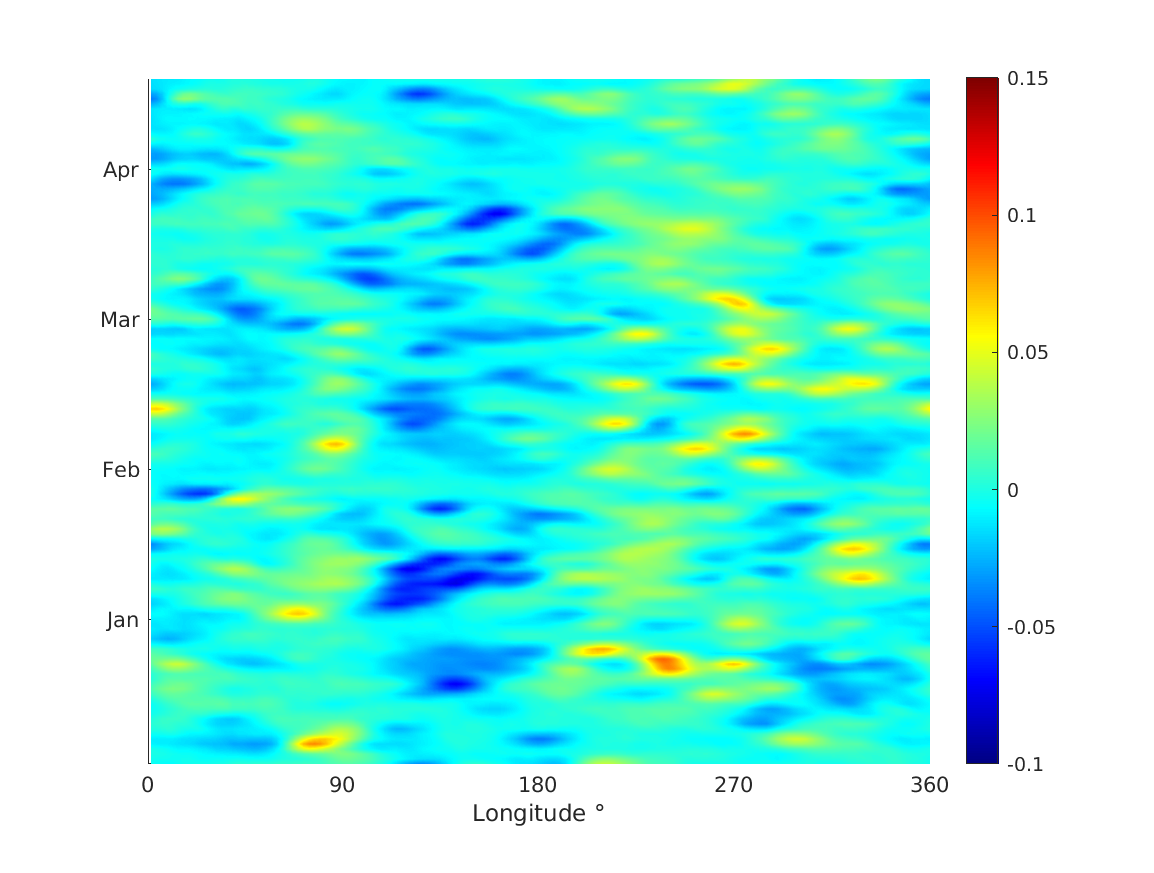
\includegraphics[width=1\textwidth]{images/M1_rec_5.eps}
\end{minipage}}
\subfigure[Joint process kriging $\mathcal{M}_{2}$]{
\begin{minipage}[t]{0.3\textwidth}
 \centering
  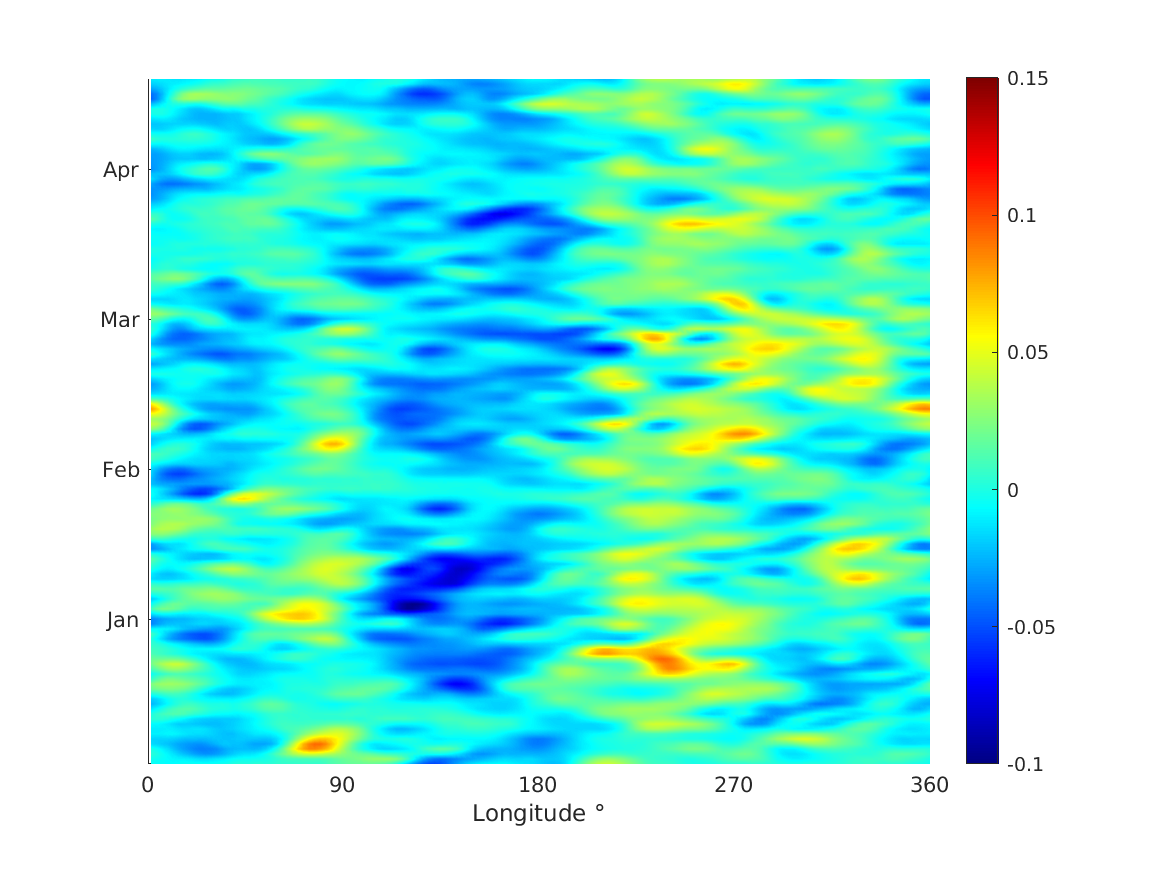
\includegraphics[width=1\textwidth]{images/M2_rec_5.eps}
\end{minipage}}
\subfigure[Joint independent kriging $\mathcal{M}_{\mathrm{ind}}$]{
\begin{minipage}[t]{0.3\textwidth}
  \centering
  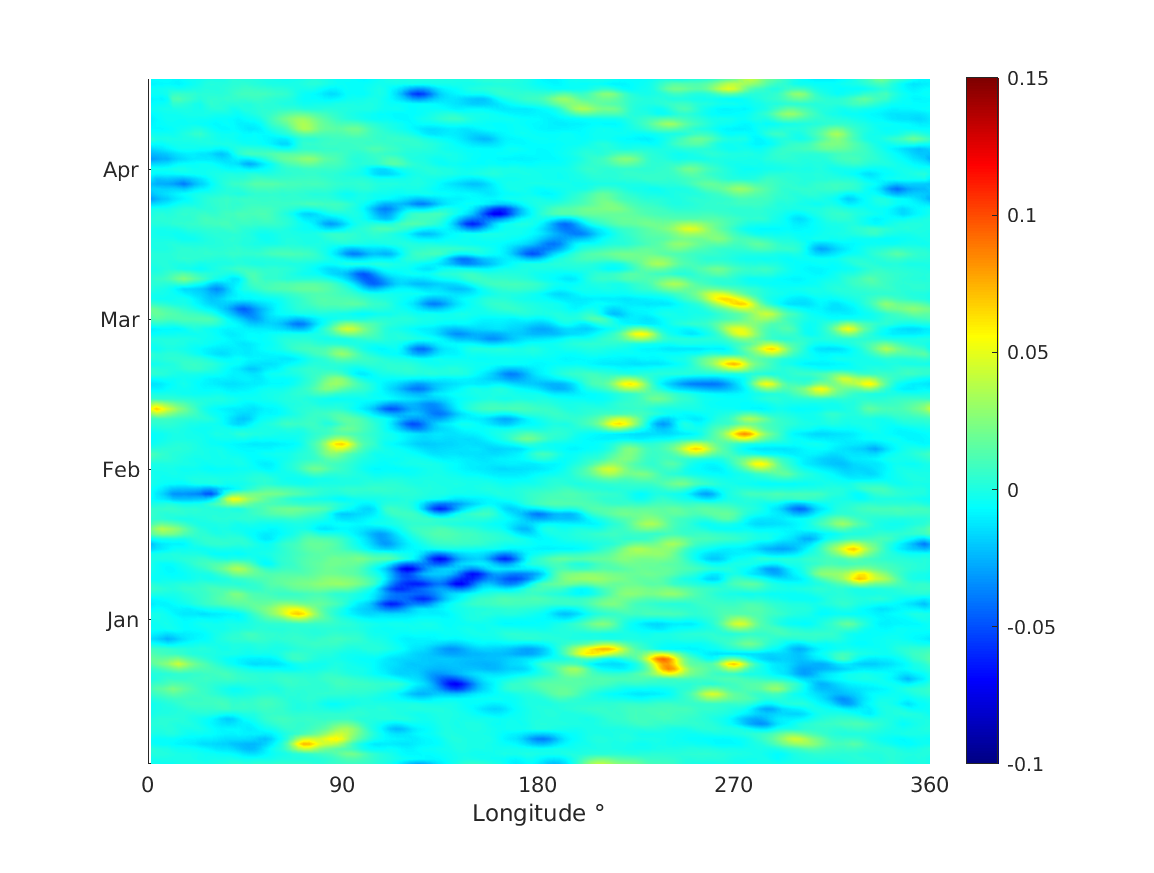
\includegraphics[width=1\textwidth]{images/M4_rec_5.eps}
  \end{minipage}}
  \caption{Predictions corresponding to (a) latent process kriging $\mathcal{M}_{1}$, (b) joint process kriging $\mathcal{M}_{2}$, and (c) joint independent kriging $\mathcal{M}_{\mathrm{ind}}$. The time period is from Dec. 1, 1982, to April 18, 1983. Both datasets are nondimensional.}\label{fig:5}
\end{figure}

\begin{figure}[!t]
\centering
\subfigure[Error histograms $\mathcal{M}_{1}$ vs. $\mathcal{M}_{\mathrm{ind}}$]{
\begin{minipage}[t]{0.3\textwidth}
 \centering
  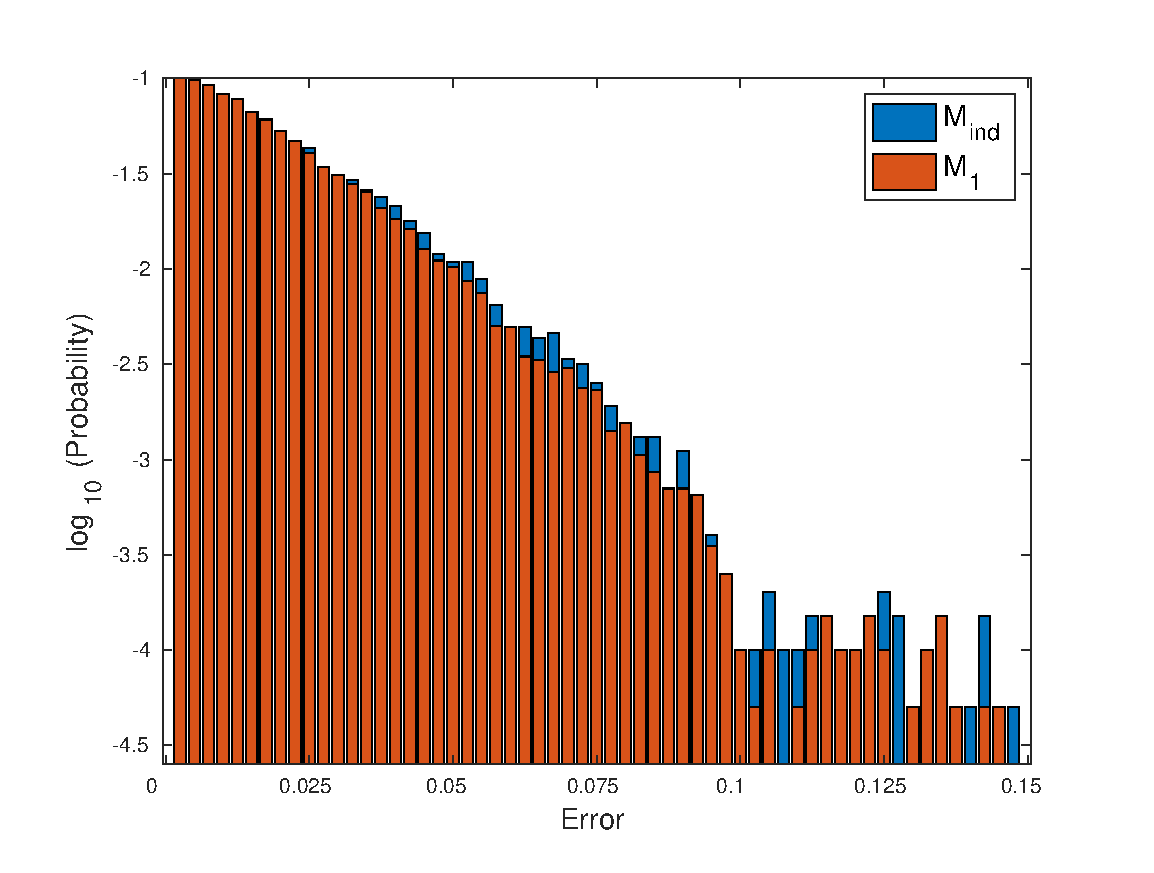
\includegraphics[width=1\textwidth]{images/M1_M4_hist_log.eps}
\end{minipage}}
\subfigure[Error histograms $\mathcal{M}_{2}$ vs. $\mathcal{M}_{\mathrm{ind}}$]{
\begin{minipage}[t]{0.3\textwidth}
 \centering
  \includegraphics[width=1\textwidth]{images/M2_M4_hist_log.eps}
\end{minipage}}
  \caption{Error histograms corresponding to independent process kriging $\mathcal{M}_{\mathrm{ind}}$ and joint process kriging $\mathcal{M}_{2}$. Note that the vertical axis represents the probability densities in logarithmic scale. The logarithm of zero density has been truncated to meet the base value of each bar plot.}\label{fig:6}
\end{figure}


We conclude that in this case the physics-based model produces a moderate improvement in prediction with this real dataset. We have tried other configurations; and while the physics-based cross-correlation model was consistently better than the independent model, the improvement seemed not particularly significant in several cases. Several areas for improvement remain here, such as considering less smooth covariance kernels (at the price of increasing the rank of the approximation or even changing the approximation strategy) and datasets with greater large-scale variability or more pronounced nonlinear effects. 

We note, however, that the computational performance was approximately linear with the number of data points and that the statistical performance was comparable to the one of exactly computed models that had far more intense computational requirements. We conclude that our approach of a physics-based implicitly defined kernel using our scalable approximation method brings a notable methodological improvement for real datasets in that it is scalable as opposed to the classical approach and that it sometimes leads to noticeable improvements in the statistical performance. 

\section{Discussion}\label{sec6}
\par Gaussian processes(GPs) are powerful tools in statistical modeling. In that space, the covariance structure takes a critical role in forecast accuracy and efficiency. Few pointers exist, however, on how to design good covariance kernels for complex processes. On the other hand, many phenomena in the natural sciences such as physics, biology, Earth science, and chemistry have been well studied, and mathematical or physical models have been established to interpret the underlying relations among the variables. Including such information from the physical models when constructing the covariance structure can be meaningful for forecasts when performing inferences on processes with partially known physical relations. One drawback of GPs, however, is that their classical computational approach, based on the Cholesky factorization of an often dense kernel, scales cubically with the number of observations. For large datasets, a reduction in the computational cost is necessary before such methods become practical.

\par In this work, we utilized physics-based, implicitly defined covariance models and present a low-rank approximation of the covariance matrix that allows the GP regression and the MLE to be conducted in quasilinear time scale. The implicitly defined nature of the kernel gives significant flexibility to the user who needs only access to a coarse physical model represented by a forward solver. Moreover, we  proposed a method to approximate the expected Fisher information matrix for quantifying the uncertainties of the estimates. Furthermore, we proposed approaches to include higher-order terms in auto-covariance matrices that are essential for describing nonlinear processes while maintaining quasilinear scaling. In summary, we presented a coherent framework for efficiently interpolating the random field and produced uncertainty estimates of this task by means of partial observations and exploiting approximate physical relationships. We presented several numerical experiments that demonstrate the accuracy of the approximated MLE by showing that the approximated parameter estimates and the uncertainties are relatively close to the exact values when the latter are known. Then we used the estimated parameters in the physics-based covariance models and demonstrated that a covariance model that is complete and has correct physically consistent structure yields significant improvements in forecasts accuracy and efficiency. We  applied the framework to real climate data to further illustrate the effectiveness of our algorithms.

\par Our approach is implicit in that it requires only a black-box forward solver of the approximate physical relationships, making the extension of the algorithm to other models immediate.  This feature increases the flexibility of the approach, benefiting from plentiful well-studied numerical discretization schemes and well-established simulation toolkits for solving physical models. Also our approach consists of independent calls to the solver that can fully take advantage of the parallel computing capability of modern hardware. 

\par Our approach does have several shortcomings.  Our approximations of the gradient and Hessian can be accurate under certain regularity conditions of the physical model. For nondifferentiable or even discontinuous models, however, the approximations can be inefficient, making the approach case-dependent. Perhaps more problematic is the fact that we apply the approach to noise kernels that are very smooth. While this is a common choice, in many cases it may not be appropriate, and we need to change the approximation method. We chose the Chebyshev interpolation method because it is simple to implement and the compressed covariance matrix is differentiable, but this can be improved by using the Nystr\"{o}m method and its variants \cite{Nystrom1,Nystrom2}, hierarchical matrix approximations \cite{Hier1,BormApproximating}, or adaptive low-rank approximations \cite{AdaptiveLowRank1,AdaptiveLowRank2}. In any case, simple global low-rank approximations like the ones we used here work well for covariance functions that are sufficiently smooth and dominated by long-range relationships between data points. When the covariance function changes more rapidly, global low-rank methods cannot capture the variability and other methods, such as hierarchical matrix approximations \cite{Hier1,BormApproximating}, may be needed. 

\section*{Acknowledgment}
This material is based upon work
supported by the U.S. Department of Energy, Office of Science,
Office of Advanced Scientific Computing Research (ASCR) under
Contract DE-AC02-06CH11357 and by NSF
through award CNS-1545046. 

\newpage
\appendix
\section{Joint Process Kriging with Higher-Order Terms}\label{App:jpf}

\begin{algorithm}[h!]
\caption{Joint Process Kriging with Higher-Order Terms $\mathcal{M}_{2}^{+}$}\label{alg:6}
Use the low-rank approximation with $N=O(\log{n})$. Specifically, $\mathrm{Cov}(z_{o},z_{o})\approx C_{z_{o}}^{T}KC_{z_{o}},\mathrm{Cov}(z_{o},z)\approx C_{z_{o}}^{T}KC_{z},\mathrm{Cov}(z_{p},z)\approx C_{z_{p}}^{T}KC_{z},\mathrm{Cov}(z_{p},z_{o})\approx C_{z_{p}}^{T}KC_{z_{o}}$.\\
%\begin{algorithmic}[1]
\textit{Step 1.} Compute $A_{1}=L_{o}C_{z}^{T}\in\mathbb{R}^{d\times N}$, $A_{2}=L_{p}C_{z}^{T}\in\mathbb{R}^{(m-d)\times N}$ by $O(N)$ forward solves.\\
\textit{Step 2}. Compute the Cholesky factorization $K=P^{T}P$, which takes $O(N^{3})$ time.\\
\textit{Step 3}. Draw $2N_{l}$ independent Rademacher vectors $\{u_{i}\}$,$\{v_{i}\} \in \mathbb{R}^N$, $i=1,2,\ldots,N_l$. Compute
\begin{align}
    \phi_{i}=C_{z}^{T}P^{T}u_{i}, \psi_{i}=C_{z}^{T}P^{T}v_{i}.
\end{align}
This takes $O(2N_{l}(N^{2}+nN))$ time.\\
\textit{Step 4}. Compute vector-Hessian-vector product by approximation (\ref{eq15}). This approximation takes $O(N_{l})$ forward solves. Denote $w_{i}=\psi_{i}^{T}H_{o}\phi_{i}$, $w_{i}'=\psi_{i}^{T}H_{p}\phi_{i}$. Then set the matrices $A_{3}\gets \frac{1}{\sqrt{2N_{l}}}(w_{1},w_{2},\cdots,w_{N_{l}})\in\mathbb{R}^{d\times N_{l}}$, $A_{4}\gets \frac{1}{\sqrt{2N_{l}}}(w_{1}',w_{2}',\cdots,w_{N_{l}}')\in\mathbb{R}^{(m-d)\times N_{l}}$. Using \eqref{eq33}, we will approximate higher-order terms by
\begin{align}
    \frac{1}{2}{\rm{tr}}(H_{o}{\rm{Cov(z,z)}}H_{o}^{T}{\rm{Cov(z,z)}})\approx A_{3}A_{3}^{T},\\
    \frac{1}{2}{\rm{tr}}(H_{p}{\rm{Cov(z,z)}}H_{o}^{T}{\rm{Cov(z,z)}})\approx A_{4}A_{3}^{T}.
\end{align}\\
\textit{Step 5}. Carry out the kriging computation \eqref{eq:jntnlnkrg} with components \eqref{eq:jntnlnk11} and \eqref{eq:jntnlnk21} in two steps. First, solve the modified inverse problem
\begin{align}
    \alpha=&\left(\begin{pmatrix}K_{\epsilon_{y}}&0\\0&K_{\epsilon_{z}}\end{pmatrix}+\begin{pmatrix}A_{3}A_{3}^{T}&0\\0&0\end{pmatrix}+\begin{pmatrix}A_{1}&0\\0&C_{z_{o}}^{T}\end{pmatrix}\begin{pmatrix}K&K\\K&K\end{pmatrix}\begin{pmatrix}A_{1}^{T}&0\\0&C_{z_{o}}\end{pmatrix}\right)^{-1}\begin{pmatrix}y_{o}-m(y_{o})\\z_{o}-m(z_{o})\end{pmatrix},\notag\\
    =&\left(\begin{pmatrix}K_{\epsilon_{y}}&0\\0&K_{\epsilon_{z}}\end{pmatrix}+\begin{pmatrix}A_{3}&A_{1}P^{T}\\0&C_{z_{o}}^{T}P^{T}\end{pmatrix}\begin{pmatrix}A_{3}^{T}&0\\PA_{1}^{T}&PC_{z_{o}}\end{pmatrix}\right)^{-1}\begin{pmatrix}y_{o}-m(y_{o})\\z_{o}-m(z_{o})\end{pmatrix}
\end{align}
by applying the SMW formula. The time cost is dominated by computing the matrix products $\begin{pmatrix}A_{3}^{T}&0\\PA_{1}^{T}&PC_{z_{o}}\end{pmatrix}\begin{pmatrix}K_{\epsilon_{y}}^{-1}&0\\0&K_{\epsilon_{z}}^{-1}\end{pmatrix}\begin{pmatrix}A_{3}&A_{1}P^{T}\\0&C_{z_{o}}^{T}P^{T}\end{pmatrix}$, which take $O(N+N_{l})$ linear system solves with the observation noise matrix  and $O((n+m)(N+N_{l})^{2})$ assembly time.\\
\textit{Step 6}. \textbf{Return} the final solution
\begin{align}
    \begin{pmatrix}m(y_{p})\\m(z_{p})\end{pmatrix}+\left(\begin{pmatrix}A_{4}A_{3}^{T}&0\\0&0\end{pmatrix}+\begin{pmatrix}A_{2}&0\\0&C_{z_{p}}^{T}\end{pmatrix}\begin{pmatrix}K&K\\K&K\end{pmatrix}\begin{pmatrix}A_{1}^{T}&0\\0&C_{z_{o}}\end{pmatrix}\right)\alpha,
\end{align}
by matrix-vector product. It takes $O(2(n+m)N+2mN_{l}+4N^{2})$ time.
%\end{algorithmic}
\end{algorithm}

\par In summary, based on our assumption of observation noise covariance matrices, the entire approach takes $O(N+N_{l})$ forward solves and $O(N+N_{l})$ observation noise covariance matrix linear system solves, and the dominant computational cost takes $O((m+n)(N+N_{l})^{2})$ time, although the workflow is highly parallelizable. The cost is quasilinear with $n$ if $N,N_{l}=log(n)$.

\section{Tensor Algebra Conventions}
\label{app:tac}
\par Computing the higher-order terms in the physics-based covariance model requires tensor operations. We  use the tensor algebra with the following convention throughout the paper. Assume the vector-valued function F(z) defines a mapping $\mathbb{R}^{n}\rightarrow \mathbb{R}^{m}$ and the Jacobian is an $m\times n$ matrix where each entry $L_{ij}=\frac{\partial F_{i}(z)}{\partial z_{j}}$. The Hessian of $F$ is a rank-three tensor $H$. We arrange the order of indices of the tensor by $H_{ijk}=\frac{\partial^{2}F_{j}(z)}{\partial y_{i}\partial y_{k}}$. Therefore, $H$ is a $n\times m\times n$ tensor. The Hessian tensor can be viewed as an array of Hessian matrices of each components of the function
\begin{align}
    H=\begin{pmatrix}H_{1}\\ \vdots\\H_{m}\end{pmatrix},\label{eqb1}
\end{align}
where each $H_{i}\in\mathbb{R}^{n\times n}$ is the symmetric Hessian matrix of the $i$th component of F. The transpose of the tensor is defined by permuting the first and last indices as well as the entire array:
\begin{align}
    H^{T}=(H_{1}^{T},H_{2}^{T},\cdots,H_{m}^{T}).\label{eqb2}
\end{align}
\par Following this convention, the tensor-tensor, tensor-vector, and tensor-matrix product can be defined in an ``elementwise sense'': for any vector $u$ and matrix $U$ of proper size, we define
\begin{align}
    Hu=\begin{pmatrix}H_{1}u\\ \vdots\\H_{m}u\end{pmatrix},\ HU=\begin{pmatrix}H_{1}U\\ \vdots\\H_{m}U\end{pmatrix}.\label{eqb3}
\end{align}
\par Additionally, we define the following tensor-tensor product, which is useful in the quadratic form computation. Assume $\hat{H}$ is an $n\times \hat{m}\times n$ tensor,
\begin{align}
    HU\hat{H}^{T}U=\begin{pmatrix}H_{1}U\hat{H}_{1}^{T}U & \cdots & H_{1}U\hat{H}_{\hat{m}}^{T}U\\\vdots & \ddots & \vdots\\H_{m}U\hat{H}_{1}^{T}U & \cdots & H_{m}U\hat{H}_{\hat{m}}^{T}U\end{pmatrix}.\label{eqb4}
\end{align}
\par The left multiplications are defined in the same elementwise sense, with left multiplications in each entry instead. As a result, bilinear forms of such tensors on vectors $u,v, \in \mathbb{R}^m$ become a contraction along indices 1,3, and thus the vector
\begin{align}
v^THu=\begin{pmatrix}v^TH_{1}u\\ \vdots\\v^T H_{m}u\end{pmatrix} \in \mathbb{R}^m. \label{eqb5}
\end{align}
\par The trace operation of the rank-three tensor is a tensor contraction to a vector taking over the first and last indices defined by
\begin{align}
    \mathrm{tr}(H)=[(\sum_{i,k}H_{ijk}\delta_{ik})_{j}]=\begin{pmatrix}\mathrm{tr}(H_{1})\\ \vdots\\\mathrm{tr}(H_{m})\end{pmatrix}.\label{eqb6}
\end{align}
\par In particular, the trace of a rank-four tensor of form \eqref{eqb4} can be defined:
\begin{align}
    \mathrm{tr}(HU\hat{H}^{T}U)=\begin{pmatrix}\mathrm{tr}(H_{1}U\hat{H}_{1}^{T}U) & \cdots & \mathrm{tr}(H_{1}U\hat{H}_{\hat{m}}^{T}U)\\\vdots & \ddots & \vdots\\\mathrm{tr}(H_{m}U\hat{H}_{1}^{T}U) & \cdots & \mathrm{tr}(H_{m}U\hat{H}_{\hat{m}}^{T}U)\end{pmatrix}\in\mathbb{R}^{m\times \hat{m}}.\label{eqb7}
\end{align}

\section{Derivation of Higher-Order Terms} \label{s:hot}
\par Here the expectation of the quadratic form of centered multivariate Gaussian random variable is extensively used. Since $\delta z\in\mathbb{R}^{n}$ is a mean 0 Gaussian random variable, we have the following important properties \cite{brookes2005matrix}: For any $n\times n$ symmetric matrix $A,B$,
\begin{align}
    &\mathrm{E}(\delta z^{T}A\delta z)=\mathrm{tr}(A\mathrm{Cov}(z,z))\label{eqc1}\\
    &\mathrm{E}[(\delta z^{T}A\delta z)(\delta z^{T}B\delta z)]=2\mathrm{tr}(A\mathrm{Cov}(z,z)B\mathrm{Cov}(z,z))+\mathrm{tr}(A\mathrm{Cov}(z,z))\mathrm{tr}(B\mathrm{Cov}(z,z)).\label{eqc2}
\end{align}

\begin{proof}
Since $\delta z$ is a mean zero multivariate random variable,
\begin{align}
    \mathrm{E}(\delta z^{T}A\delta z)&=\mathrm{E}(\mathrm{tr}(\delta z^{T}A\delta z))\notag\\
    &=\mathrm{E}(\mathrm{tr}(A\delta z\delta z^{T}))\notag\\
    &=\mathrm{tr}(A\mathrm{E}(\delta z\delta z^{T}))\notag\\
    &=\mathrm{tr}(A\mathrm{Cov}(z,z)).\label{eqc3}
\end{align}
\par For Equation \eqref{eqc2}, we start from a simpler case. Assume $x\in \mathbb{R}^{n}$ is a standard normal random vector $x_{i}\sim \mathcal{N}(0,1)$ i.i.d. We first consider for any symmetric $n\times n$ matrices $\tilde{A},\tilde{B}$, 
\begin{align}
    \mathrm{E}(x^{T}\tilde{A}xx^{T}\tilde{B}x)&=\mathrm{E}\left(\sum_{i,j,k,l=1}^{n}\tilde{A}_{ij}\tilde{B}_{kl}x_{i}x_{j}x_{k}x_{l}\right)\notag\\
    &=\mathrm{E}\left(\sum_{i\neq j}\tilde{A}_{ii}\tilde{B}_{jj}x_{i}^{2}x_{j}^{2}\right)+\mathrm{E}\left(\sum_{i\neq j}\tilde{A}_{ij}\tilde{B}_{ij}x_{i}^{2}x_{j}^{2}\right)+\mathrm{E}\left(\sum_{i\neq j}\tilde{A}_{ij}\tilde{B}_{ji}x_{i}^{2}x_{j}^{2}\right)+\mathrm{E}\left(\sum_{i=1}^{n}\tilde{A}_{ii}\tilde{B}_{ii}x_{i}^{4}\right)\notag\\
    &=\mathrm{E}\left(\sum_{i\neq j}\tilde{A}_{ii}\tilde{B}_{jj}\right)+2\mathrm{E}\left(\sum_{i\neq j}\tilde{A}_{ij}\tilde{B}_{ji}\right)+3\mathrm{E}\left(\sum_{i=1}^{n}\tilde{A}_{ii}\tilde{B}_{ii}\right).\label{eqc4}
\end{align}
\par Note that the last step comes from the fact that $\tilde{B}$ is a symmetric matrix and the Isserlis' theorem. On the other hand, note that
\begin{align}
    &\mathrm{tr}(\tilde{A}\tilde{B})=\sum_{i,j=1}^{n}\tilde{A}_{ij}\tilde{B}_{ji}=\sum_{i\neq j}^{n}\tilde{A}_{ij}\tilde{B}_{ji}+\sum_{i=1}^{n}\tilde{A}_{ii}\tilde{B}_{ii}\label{eqc5}\\
    &\mathrm{tr}(\tilde{A})\mathrm{tr}(\tilde{B})=\sum_{i\neq j}^{n}\tilde{A}_{ii}\tilde{B}_{jj}+\sum_{i=1}^{n}\tilde{A}_{ii}\tilde{B}_{ii}.\label{eqc6}
\end{align}
\par Comparing \eqref{eqc4} with \eqref{eqc5} and \eqref{eqc6},  we have
\begin{align}
    \mathrm{E}(x^{T}\tilde{A}xx^{T}\tilde{B}x)=2\mathrm{tr}(\tilde{A}\tilde{B})+\mathrm{tr}(\tilde{A})\mathrm{tr}(\tilde{B}).\label{eqc7}
\end{align}
\par Now since $\delta z$ is a mean zero multivariate normal vector, there exists a matrix $L$ such that $\mathrm{Cov}(z,z)=LL^{T}$ and $\delta z=Lx$. Using \eqref{eqc7}, we have
\begin{align}
    \mathrm{E}[(\delta z^{T}A\delta z)(\delta z^{T}B\delta z)]&=\mathrm{E}[(x^{T}(L^{T}AL)x)(x^{T}(L^{T}BL)x)]\notag\\
    &=2\mathrm{tr}(L^{T}ALL^{T}BL)+\mathrm{tr}(L^{T}AL)\mathrm{tr}(L^{T}BL)\notag\\
    &=2\mathrm{tr}(ALL^{T}BLL^{T})+\mathrm{tr}(ALL^{T})\mathrm{tr}(BLL^{T})\notag\\
    &=2\mathrm{tr}(A\mathrm{Cov}(z,z)B\mathrm{Cov}(z,z))+\mathrm{tr}(A\mathrm{Cov}(z,z))\mathrm{tr}(B\mathrm{Cov}(z,z)).\label{eqc8}
\end{align}
\par We thus have proved \eqref{eqc2}.

\end{proof}

\par Following our convention of tensor algebra for Hessian tensor $H$, we get
\begin{align}
    \overline{\delta z^{T}H\delta z}&=\mathrm{E}(\delta z^{T}H\delta z)\notag\\
    &=\begin{pmatrix}\mathrm{E}(\delta z^{T}H_{1}\delta z)\\\vdots\\\mathrm{E}(\delta z^{T}H_{m}\delta z)\end{pmatrix}\notag\\
    &=\begin{pmatrix}\mathrm{tr}(H_{1}\mathrm{Cov}(z,z))\\\vdots\\\mathrm{tr}(H_{m}\mathrm{Cov}(z,z))\end{pmatrix}\notag\\
    &=\mathrm{tr}(H\mathrm{Cov}(z,z)).\label{eqc9}
\end{align}
\par Then for Hessian tensors $H\in\mathbb{R}^{n\times m\times n},\hat{H}\in\mathbb{R}^{n\times \hat{m}\times n}$,
\begin{align}
    \overline{\delta z^{T}H\delta z}\ \overline{\delta z^{T}\hat{H}^{T}\delta z}=\mathrm{tr}(H\mathrm{Cov}(z,z))\mathrm{tr}(\hat{H}\mathrm{Cov}(z,z))^{T}.\label{eqc10}
\end{align}
\par We thus have
\begin{align}
    \overline{\delta z^{T}H\delta z \delta z^{T}\hat{H}^{T}\delta z}&=\begin{pmatrix}\mathrm{E}(\delta z^{T}H_{1}\delta z \delta z^{T}\hat{H}_{1}^{T}\delta z) & \cdots & \mathrm{E}(\delta z^{T}H_{1}\delta z \delta z^{T}\hat{H}_{\hat{m}}^{T}\delta z)\\\vdots & \ddots & \vdots\\\mathrm{E}(\delta z^{T}H_{m}\delta z \delta z^{T}\hat{H}_{1}^{T}\delta z) & \cdots & \mathrm{E}(\delta z^{T}H_{m}\delta z \delta z^{T}\hat{H}_{\hat{m}}^{T}\delta z) \end{pmatrix}\notag\\
    & \stackrel{\mbox{\eqref{eqc2}}}{=}2\mathrm{tr}(H\mathrm{Cov}(z,z)\hat{H}^{T}\mathrm{Cov}(z,z))+\mathrm{tr}(H\mathrm{Cov}(z,z))\mathrm{tr}(\hat{H}\mathrm{Cov}(z,z))^{T}.\label{eqc11}
\end{align}



\bibliographystyle{IJ4UQ_Bibliography_Style}

\bibliography{References}

\vspace{0.1cm}
\begin{flushright}
	\scriptsize \framebox{\parbox{2.5in}{Government License: The
			submitted manuscript has been created by UChicago Argonne,
			LLC, Operator of Argonne National Laboratory (``Argonne").
			Argonne, a U.S. Department of Energy Office of Science
			laboratory, is operated under Contract
			No. DE-AC02-06CH11357.  The U.S. Government retains for
			itself, and others acting on its behalf, a paid-up
			nonexclusive, irrevocable worldwide license in said
			article to reproduce, prepare derivative works, distribute
			copies to the public, and perform publicly and display
			publicly, by or on behalf of the Government. The Department of Energy will provide public access to these results of federally sponsored research in accordance with the DOE Public Access Plan. http://energy.gov/downloads/doe-public-access-plan. }}
	\normalsize
\end{flushright}

\end{document}
























\section{Introduction}
Heat is difficult to measure, even at macroscales! At macroscales, key
quantities of interest for heat transfer are temperature, heat flux, and
thermophysical properties such as thermal conductivity, specific heat, etc.
Conductive and convective heat transfer at macroscale are usually governed
by diffusion processes because heat carriers (molecules, electrons, phonons,
etc.) in these processes have short mean free paths and short wavelengths.
In micro- and nanostructures, however, the mean free paths and even
wavelengths of heat carriers become comparable or longer than the
characteristic length involved in the transport process. Heat transfer can no longer be
described by established theories applicable to macroscale. It is precisely
these deviations from continuum that have drawn significant interests from
scientific communities to understand micro-/nanoscale heat transfer.
Such understandings have potential impacts over a wide range of
applications, from microelectronics to energy conversion. Experimentally
probing heat transfer in micro-/nanostructures is essential for scientific
and technological endeavors, and significant progress has been made over the
last two decades. This volume aims to provide a summary of the advances made
in probing micro-/nanoscale heat transfer.
\begin{equation}
  R(E) = \frac{\kappa}{2\eta} \int_{\Omega}\left( \nabla{E}\cdot\nabla{E} +
  \varepsilon \right)^{\eta} \, d\Omega
\end{equation}



In many \textit{gasoline direct injection} (GDI) {\it engines hollow cone} sprays generated by swirl or outwardly opening injectors are applied. In this study the spray of an outwardly opening injector is investigated. According to the geometrical shape of an outwardly opening pintle nozzle the fuel exits from an annular gap. Previous investigations have already shown that the hollow cone spray leaving this nozzle is composed of many single strings instead of a continuous conical sheet.

\section{Problem definition}
\label{sec:ProblemDef} In this section, we follow the notation
in~\cite{Xiang,Ghanem}.  Define a complete probability space
$(\Omega,\mathcal{F},\mathcal{P})$ with sample space $\Omega$ which
corresponds to the outcomes of some experiments,
$\mathcal{F}\subset 2^\Omega$ is the $\sigma$-algebra of subsets in
$\Omega$ (these subsets are called events) and
$\mathcal{P}:\mathcal{F}\rightarrow[0,1]$ is the probability
measure. Also, define $D$ as a $d$-dimensional bounded domain
$D\subset\mathbb{R}^d \ (d=1,2,3)$ with boundary $\partial D$. We
are interested to find a stochastic function $u:\Omega \times D
\rightarrow \mathbb{R}$ such that for $\mathcal{P}$-almost
everywhere (a.e.) $\omega \in \Omega$, the following equation holds:
\begin{equation}
  \mathcal{L}(\mbox{\boldmath $x$},\omega;u) = f(\mbox{\boldmath $x$},\omega),~~\forall \mbox{\boldmath $x$} \in D,
  \label{eqn:SDE}
\end{equation}
\noindent
and
\begin{equation}
  \mathcal{B}(\mbox{\boldmath $x$};u) = g(\mbox{\boldmath $x$}),~~\forall \mbox{\boldmath $x$} \in \partial D,
  \label{eqn:Boundary}
\end{equation}
\noindent
where $\mbox{\boldmath $x$} = (x_1,\dots,x_d)$ are the coordinates
in $\mathbb{R}^d$, $\mathcal{L}$ is (linear/nonlinear) differential
operator, and $\mathcal{B}$ is a boundary operator. In the most
general case, the operators $\mathcal{L}$ and $\mathcal{B}$ as well
as the driving terms $f$ and $g$, can be assumed random. We assume
that the boundary has sufficient regularity and that $f$ and $g$ are
properly defined such that the problem in
Eqs.~(\ref{eqn:SDE})--(\ref{eqn:Boundary}) is well-posed
$\mathcal{P}$ -a.e. $\omega \in \Omega$.




\subsection{The Finite-Dimensional Noise Assumption and the Karhunen-Lo\`eve
Expansion the Finite-Dimensional Noise Assumption and the Karhunen-Lo\`eve
Expansion}\label{sec:KLE} Any second-order stochastic process can be
represented as a random variable at each spatial and temporal
location. Therefore, we require an infinite number of random
variables to completely characterize a stochastic process. This
poses a numerical challenge in modeling uncertainty in physical
quantities that have spatio-temporal variations, hence necessitating
the need for a reduced-order representation (i.e., reducing the
infinite-dimensional probability space to a finite-dimensional one).
Such a procedure, commonly known as a `finite-dimensional noise
assumption' \cite{FooPhD,2006AIPC..845..479B}, can be achieved through any
truncated spectral expansion of the stochastic process in the
probability space. One such choice  is the Karhunen-Lo\`eve (K-L)
expansion \cite{Ghanem}.
\subsubsection{Suspended Structures}

Suspended structures used for nanowire
thermal conductivity measurements serve as a good example.
From the entire volume, it is clear that significant progress has been made
in experimental techniques to probe nanoscale heat transfer phenomena, and
the experimental results have led to new understandings of heat transfer
physics, generated new challenges, and opened new opportunities. From my own
perspective, the following are some significant challenges.

\paragraph{Suspended Structures}

Suspended structures used for nanowire
thermal conductivity measurements serve as a good example.
From the entire volume, it is clear that significant progress has been made
in experimental techniques to probe nanoscale heat transfer phenomena, and
the experimental results have led to new understandings of heat transfer
physics, generated new challenges, and opened new opportunities. From my own\footnote{Suspended structures used for nanowire
thermal conductivity measurements serve as a good example.}
perspective, the following are some significant challenges.

\begin{theorem}\label{un_energy}
There exists a unique solution $u_n \in L^2\left(O, H_0^1\left(D\right)\right)$ to the problem \eqref{eqn:SDE} and \eqref{eqn:Boundary} for $n=0$,
and the problem \eqref{eqn:SDE}--\eqref{un_est} for $n\geq 1$. In addition, if $f\in L^2\left(O, H^{-1+\sigma}\left(D\right)\right)$ for $\sigma\in(0,1]$, it holds that
\begin{equation}\label{un_est}
E(|{u_n}|_{H^{1+\sigma}(D)}^2) \leq  C_0^{n+1} \;E({f}_{H^{-1+\sigma}(D)}^2),
\end{equation}
for some constant $C_0$ independent of $n$ and $s$.
\end{theorem}

%\medskip

\begin{proof}
For $n=0$, the existence of the weak solutions can be deduced from the Lax-Milgram theorem,
and the desired energy estimate,
\begin{equation*}
E(|{u_0}|_{H^{1+\sigma}(D)}^2) \leq  \tilde C_0\;E({f}_{H^{-1+\sigma}(D)}^2),
\end{equation*}
This completes the proof.
\end{proof}





\begin{figure}[!b]
	\centering
  \includegraphics[width=12cm]{Fig1.eps}\\
  (a)\hspace*{200pt}(b)
\caption{Visualization setup. (a) Some description for left part. (b) Some description for right part.}
\label{fig:VisSetup}
\end{figure}
\begin{table}[!b]
\centering\begin{threeparttable}[!b]
\caption{Injected fuel mass}
\centering\begin{tabular}{|ccc|}
\hline
\textbf{Injection duration}   & \textbf{Injection pressure} & \textbf{Fuel mass}  \\
$\Delta t$ \textbf{(\textmu s)} & \textbf{(MPa)} & \textbf{(mg)} \\
\hline
300 & 1 & 1.7 \\
300 & 2 & 3.0 \\
300 & 3 & 4.0 \\
300 & 4 & 4.7 \\
300 & 5 & 5.4 \\
300 & 6 & 6.0 \\
300 & 7 & 6.5 \\
300 & 8 & 6.9 \\
300 & 9 & 7.2 \\
300 & 10 & 7.6 \\
300 & 11 & 7.7 \\
300 & 12 & 8.0 \\
\hline
100 & 10 & 0.6 \\
200 & 10 & 4.3 \\
400 & 10 & 10.3\tnote{a} \\
\hline
\end{tabular}
\small{\begin{tablenotes}[normal,flushleft]
\item [a]\hspace*{-3pt} the first note.
\end{tablenotes}}
\end{threeparttable}
\end{table}

\section{Adaptive sparse grid collocation method (ASGC)}
\label{sec:ASGC} In this section, we briefly review the development
of the ASGC strategy. For more details, the interested reader is
referred to~\cite{Xiang,KlimkePhD}.

The basic idea of this method is to have a finite element
approximation for the spatial domain and approximate the
multi-dimensional stochastic space $\Gamma$ using interpolating
functions on a set of collocation points $\{\bold{Y}_i\}_{i=1}^k \in
\Gamma$.  Suppose we can find a finite element approximate solution
$u$ to the deterministic solution of the problem in
Eq.~(\ref{eqn:SDE}), we are then interested in constructing an
interpolant of $u$ by using linear combinations of the solutions
$u(\cdot,\bold{Y}_i)$. The interpolation is constructed by using the
so called sparse grid interpolation method based on the Smolyak
algorithm. In the context of incorporating adaptivity, we have
chosen the collocation point based on the Newton-Cotes formulae
using equidistant support nodes. The corresponding basis function is
the multi-linear basis function constructed from the tensor product
of the corresponding one-dimensional functions.

\begin{algorithm}[!t]
	\caption{Block-circulant embedding method (BCEM)}
	\label{alg:bcem}
Given $N\in \mathbb{Z}^d, x_\textbf{0}\in \Omega$, and strictly positive valued vector $h \in \mathbb{R}^d$,\\
	%\begin{algorithmic}
	 	\textit{Step 1}. Choose a vector $m\in \mathbb{Z}^d$ such that $m[i] \geq 2 N[i]$ for all $1 \leq i \leq d$. \label{step01}\\
		\textit{Step 2}.  Compute the first block row of the circulant matrix $C$ as described. \label{step02}\\
		\textit{Step 3}.  Compute the block-diagonal matrix $\Lambda = \mathrm{diag}(\Lambda_0, \cdots,\Lambda_{\overline{m}-1})$. \label{step03}
	%\end{algorithmic}
\end{algorithm}



Any function $f \in \Gamma$ can now be approximated by the following
reduced form:
\begin{equation}
 f\big(\mbox{\boldmath $x$},\bold{Y}\big ) = \sum _{\|{\bf i}\|\leqslant N+q} \sum_{\bold {j}}
w_{\bf j}^{\bf i}(\mbox{\boldmath $x$}) \cdot a_{\bf j}^{\bf
i}(\bold{Y}), \label{eqn:approximate}
\end{equation}
\noindent
where the multi-index $\bold{i} = (i_1,\ldots,i_N)\in \mathbb{N}^N $, the multi-index $\bold{j} = (j_1,\ldots,j_N)\in \mathbb{N}^N$ and
$\|\bold{i}\| = i_1+\cdots+i_N$. $q$ is the sparse grid
interpolation level and the summation is over collocation points
selected in a hierarchical framework~\cite{Xiang,dol04mul}. Here, $w_{\bf
j}^{\bf i}$ is the hierarchical surplus, which is just the
difference between the function value at the current point and
interpolation value from the coarser grid. The hierarchical surplus
is a natural candidate for error control and implementation of
adaptivity.

Heat flux cross small structures such as nanowires is very tiny, and
high-sensitivity heat flux meters are needed for thermal measurements.
Similar to macroscale heat flux measurements, nanoscale heat flux
measurements usually require knowing temperature differences between two
points and thermal resistance between the same points, from which the heat
flux can be calculated. The key for small heat flux measurements is to
create structures with large thermal resistance values between the two
temperature measurements points.




\section{Conclusions}

Significant progress has been made in terms of tailoring the radiative
properties with micro-/nanost\-ructured materials. Rapid developments have
been made in fabricating periodic gratings and nanostructured periodic
arrays of metal materials over thin films and multilayers. Magnetic
responses have been demonstrated in the infrared and even visible spectral
regions. Further research is needed to understand the coupling mechanisms
between various modes and localized surface plasmons. While FDTD and RCWA
can be used to calculate the radiative properties for engineered surfaces
with micro-/nanostructures, faster computational algorithms are needed with
complicated structures to assist the design for specific applications. The
optical constants are often different in the nanostructured materials as
compared with the bulk solid. Furthermore, for high-temperature
applications, the chemical and thermal stability must be considered, as well
as the size- and temperature-dependent optical constants of the materials.
\begin{enumerate}
  \item Aligned metallic nanowires may exhibit unique optical and thermal radiative
properties due to the surface-enhanced absorption and scattering,
anisotropic dielectric function, and magnetic resonance (between parallel
wires), and may be applied to diffraction optics as well as IR polarizers
and in the control of optical and radiative properties
  \item Detailed models
considering both surface scattering and volume scattering will allow better
understanding of the radiative transfer in these inhomogeneous structures.
Methods for fabricating more uniform structures in large areas with a high
yield are still needed.
  \item Measurements at longer wavelengths, i.e., mid- to
far-IR, will help in understanding the effective medium behavior as well as
the magnetic response.
\end{enumerate}
VACNT arrays show great promise for radiometric applications as nearly
perfect absorbers and emitters in a broad spectral region. EMT appears to be
able to describe the visible and infrared properties of CNT arrays
reasonably well. Specular and diffuse black materials made of SWCNTs or
MWCNTs should be valuable for space-borne radiometric systems, high-power
laser radiometers, absolute cryogenic radiometers, and infrared calibration
facilities. The chemical stability and mechanical rigidity of these
structures also need to be further investigated.
A challenge that exists in
the materials growth process is how to control the growth conditions so that
arrays with a controllable degree of alignment and surface morphology can be
reproduced.  However, this error indicator is too sharp and may
result in a non-terminating algorithm.






%% The Acknowledgements part is started with the command \acknowledgements;
%% acknowledgements are then done as normal sections before appendix
%% \acknowledgements

\acknowledgements

This research was supported by the Computational Mathematics program of
AFOSR (grant FA9550-07-1-0139).


%% The Appendices part is started with the command \appendix;
%% appendix sections are then done as normal sections and after Acknowledgements
%% \appendix

%% \section{}
%% \label{}

%% References without bibTeX database:

%\begin{thebibliography}{-8}

%% \bibitem must have the following form:

%\small{
%\bibitem{key}

%...

%}

%\end{thebibliography}

%% References with bibTeX database:

\bibliographystyle{IJ4UQ_Bibliography_Style}

\bibliography{References}



\end{document}



\par Now to combine the data and the model, the zonal wind velocity serves as a surrogate of $u$ in the model. For $q$, the relative humidity (mixing ratio) in 500 hPa pressure level is a natural surrogate of water vapor in middle troposphere. Additionally, it is also common to estimate the water vapor using the OLR data. Since water vapor can absorb a certain range of wavelengths in OLD adding heat to the atmosphere. High concentration of water vapor tends to reduce the OLR below clear sky values. Therefore the OLR data can also be used as a surrogate of the water vapor but with a negative sign. We simulate the case where the model has multiple outputs by asking the model to output two quantities but with different signs $q_{1}=q$, $q_{2}=-q$. For $q_{1}$ and $q_{2}$ we use the relative humidity data and the OLR data respectively. Note that the real data are normalized to have the same variance as the model data before using. This differs from \cite{stechmann2017unified} where the data are nondimensionalized using the standard equatorial reference scale \cite{stechmann2015identifying} because here we use anomalies in our modified model equation. For more detailed raw data preprocessing methods please refer to \cite{stechmann2015identifying} in order to streamline our main presentation. In Figure \ref{fig:4} we show the observational relative humidity data and OLR data for all longitudes from Dec 1982 to Apr 1983 to illustrate their resemblance (but with different signs).